% !TEX root = ../main.tex
\newpage
\appendix
\section{Appendices}
\label{sec:appendices}

\plantodo{S5, S7, S10, S11 (general)}{Use appendices for material too
extensive for the main body or of interest to only some readers. Label each
lettered (Appendix A, B, ...), and ensure every appendix is referenced from
somewhere in the main body.}

\subsection{Full Nominal-Flight ConOps}
\label{app:conops}
\plantodo{S5}{Full strategic-planning through postflight/continuation
activity breakdown (see main-body summary, Section~\ref{sec:conops-results}).
The phase activity diagrams are placed below (Fly Enroute is in the body,
Figure~\ref{fig:sysml-flyEnrouteActivity}); add the text that introduces them
and cite each one from it.}

% GENERATED by tools/render_sysml_diagrams.py. Do not edit: the next run overwrites it.
% To change a caption, edit the `// caption:` line above the view in the .sysml file.
% To add or remove a figure, add or remove the view in the model.
% To move a figure between the body and the appendix, add or remove a
% `// placement: body` line above the caption line.

\begin{landscape}
\begin{figure}[!htbp]
\centering
\pdfimageresolution=300
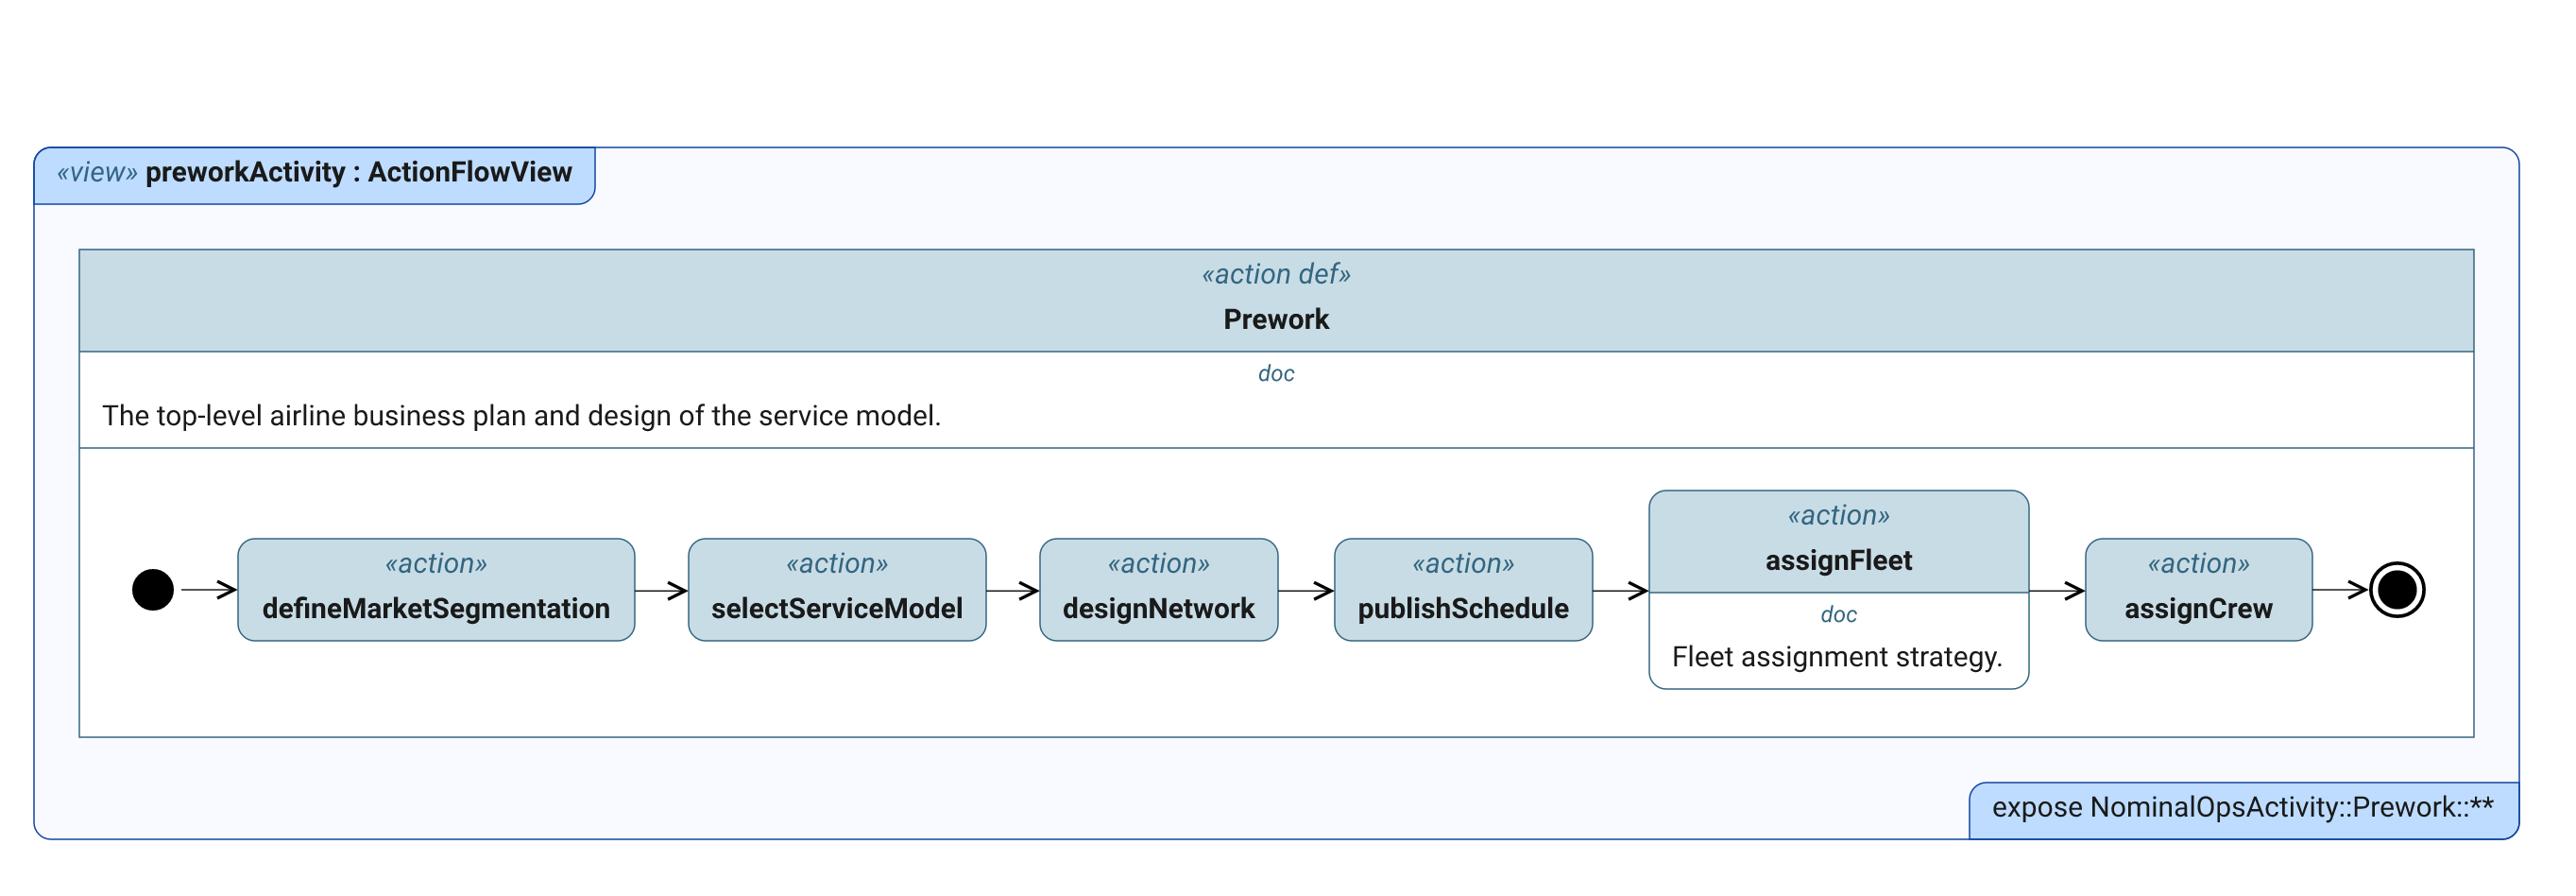
\includegraphics[width=\linewidth,height=0.8\textheight,keepaspectratio]{sysml/diagram-preworkActivity}
\caption{Nominal operations, Prework: airline planning before flight planning. View \texttt{preworkActivity}; source \texttt{nas\_activity\_diagram-nominal\_ops.sysml}; rendered 2026-10-18.}
\label{fig:sysml-preworkActivity}
\end{figure}
\end{landscape}

% GENERATED by tools/render_sysml_diagrams.py. Do not edit: the next run overwrites it.
% To change a caption, edit the `// caption:` line above the view in the .sysml file.
% To add or remove a figure, add or remove the view in the model.
% To move a figure between the body and the appendix, add or remove a
% `// placement: body` line above the caption line.

\begin{landscape}
\begin{figure}[!htbp]
\centering
\pdfimageresolution=300
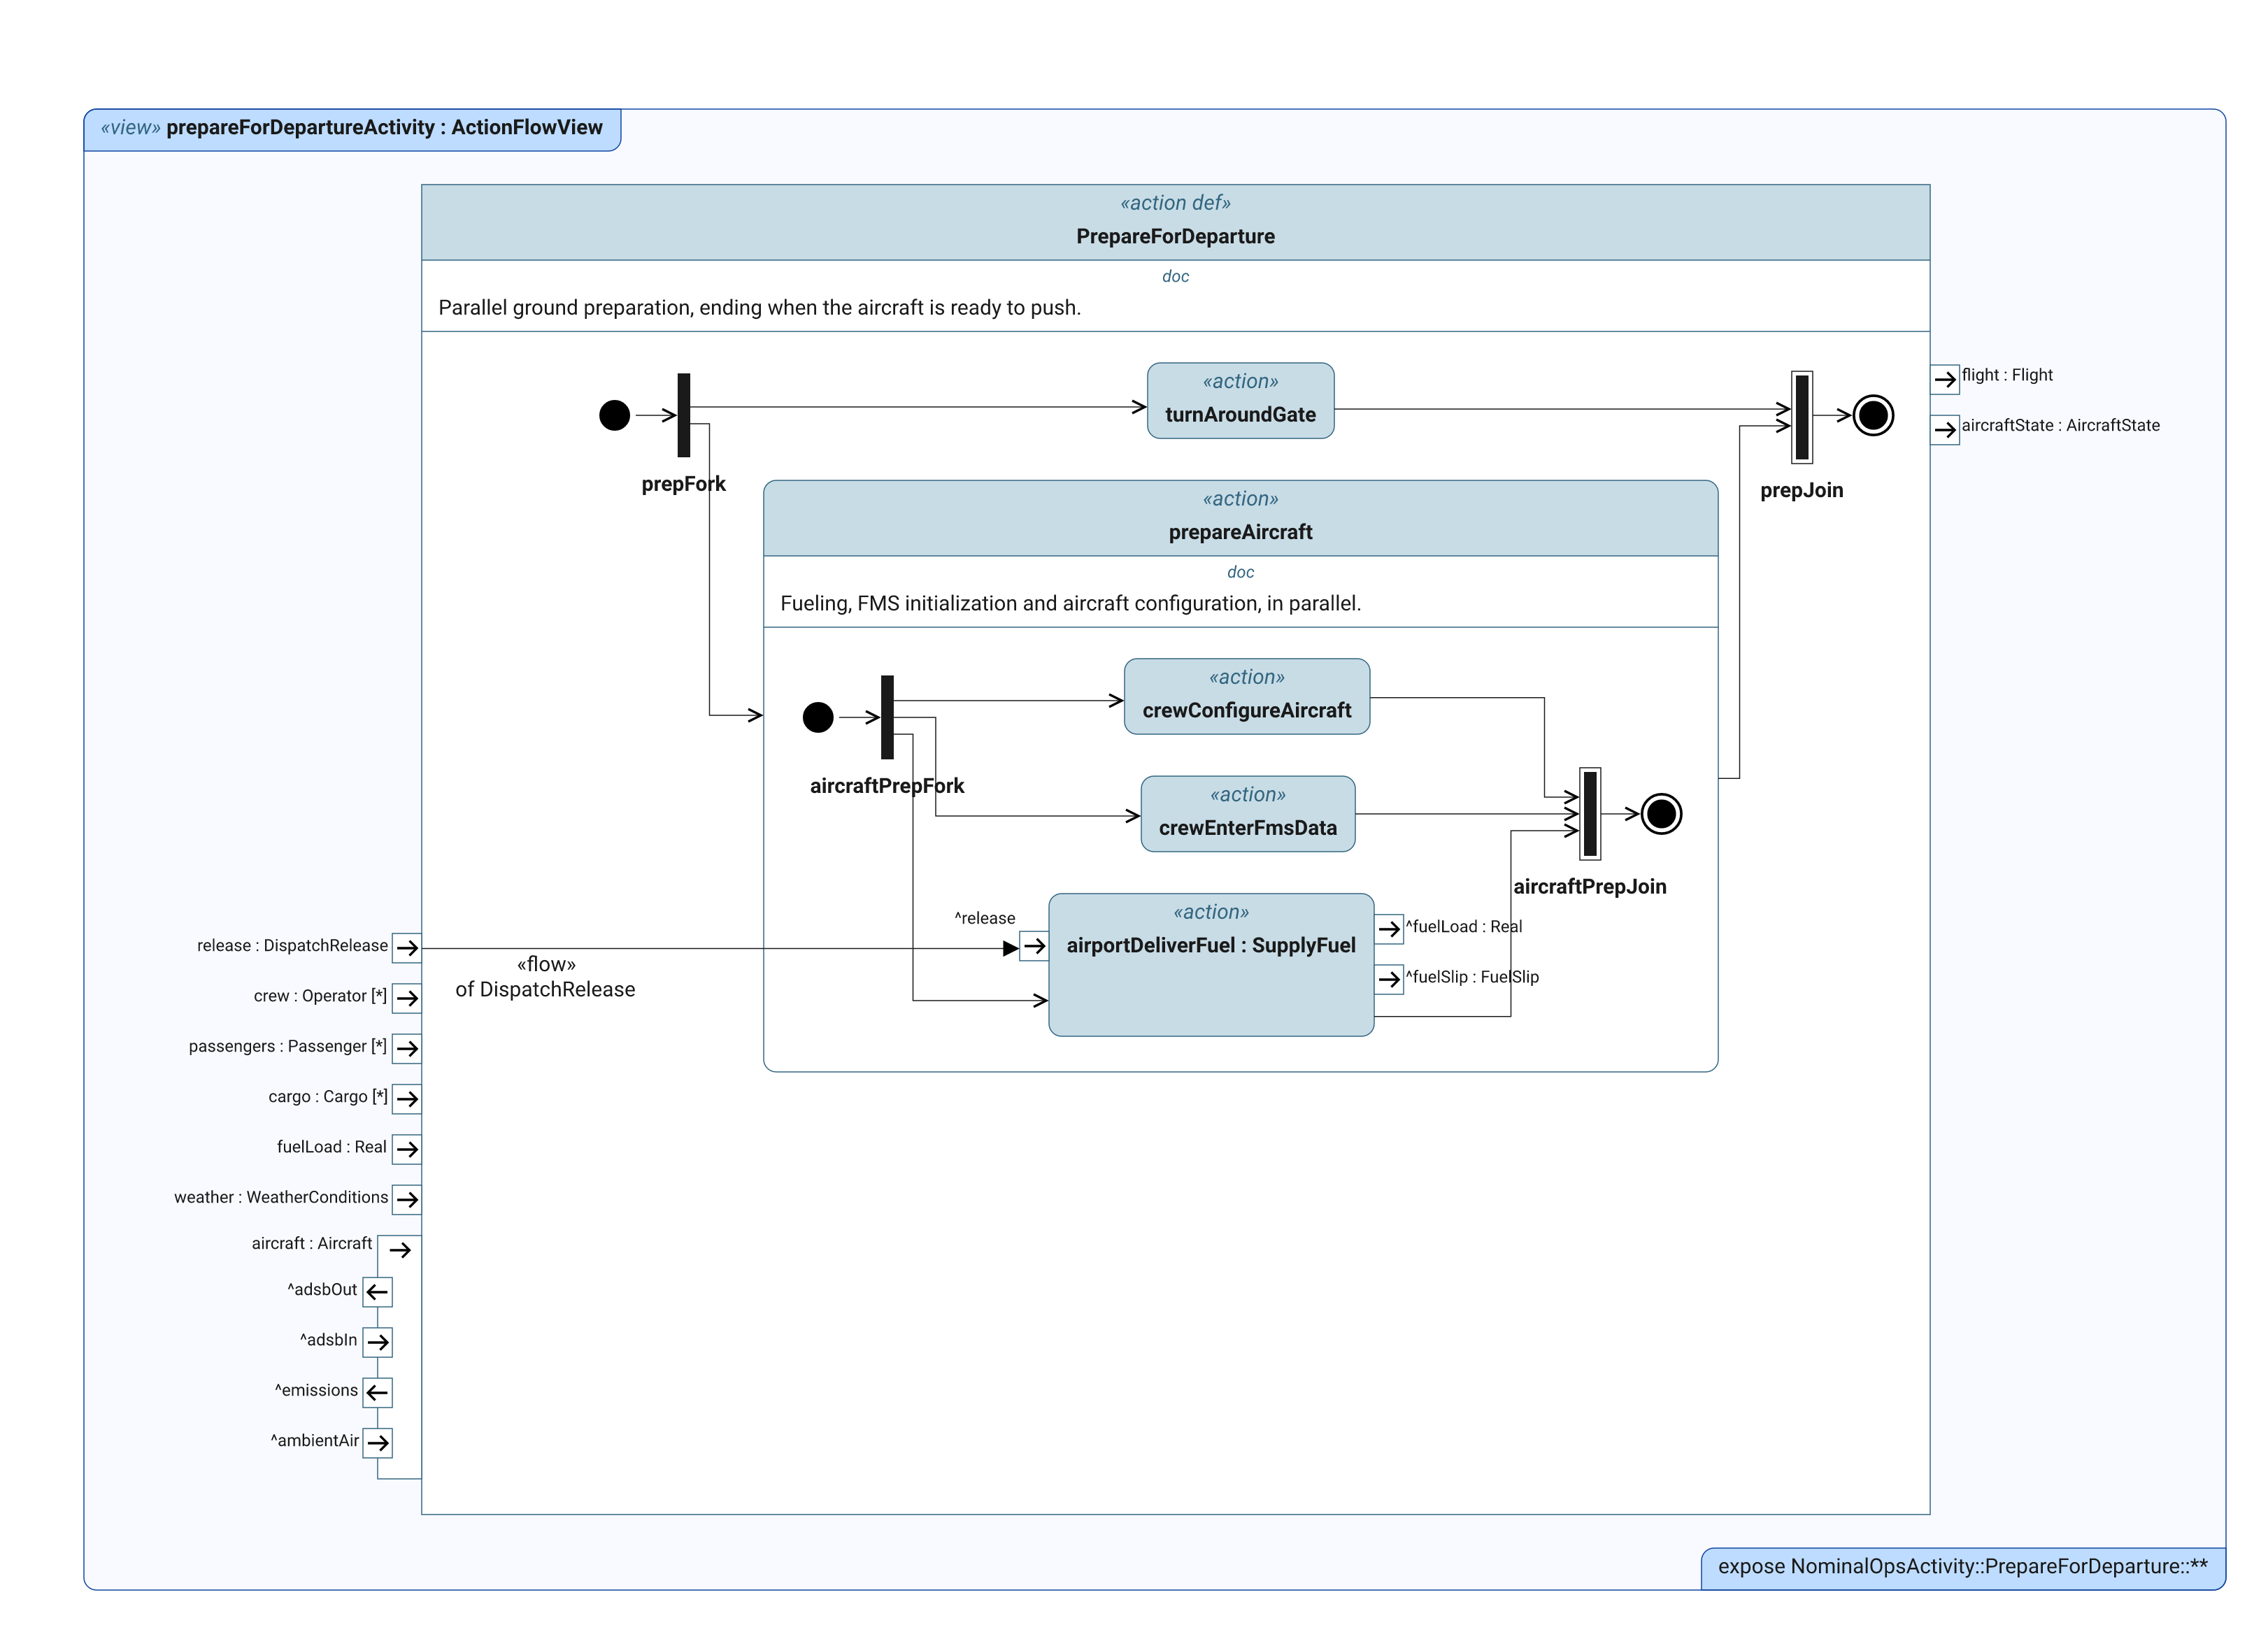
\includegraphics[width=\linewidth,height=0.8\textheight,keepaspectratio]{sysml/diagram-prepareForDepartureActivity}
\caption{Nominal operations, Prepare for Departure: parallel fueling, FMS entry, configuration and gate turnaround. View \texttt{prepareForDepartureActivity}; source \texttt{nas\_activity\_diagram-nominal\_ops.sysml}; rendered 2026-10-19.}
\label{fig:sysml-prepareForDepartureActivity}
\end{figure}
\end{landscape}

% GENERATED by tools/render_sysml_diagrams.py. Do not edit: the next run overwrites it.
% To change a caption, edit the `// caption:` line above the view in the .sysml file.
% To add or remove a figure, add or remove the view in the model.
% To move a figure between the body and the appendix, add or remove a
% `// placement: body` line above the caption line.

\begin{landscape}
\begin{figure}[!htbp]
\centering
\pdfimageresolution=300

\includegraphics[width=\linewidth,height=0.8\textheight,keepaspectratio]{sysml/diagram-departActivity}
\caption{Nominal operations, Depart: clearance, pushback, taxi-out, takeoff and climb. View \texttt{departActivity}; source \texttt{nas\_activity\_diagram-nominal\_ops.sysml}; rendered 2026-10-18.}
\label{fig:sysml-departActivity}
\end{figure}
\end{landscape}

% GENERATED by tools/render_sysml_diagrams.py. Do not edit: the next run overwrites it.
% To change a caption, edit the `// caption:` line above the view in the .sysml file.
% To add or remove a figure, add or remove the view in the model.
% To move a figure between the body and the appendix, add or remove a
% `// placement: body` line above the caption line.

\begin{landscape}
\begin{figure}[!htbp]
\centering
\pdfimageresolution=300

\includegraphics[width=\linewidth,height=0.8\textheight,keepaspectratio]{sysml/diagram-arriveActivity}
\caption{Nominal operations, Arrive: arrival planning, descent, approach, landing and taxi-in. View \texttt{arriveActivity}; source \texttt{nas\_activity\_diagram-nominal\_ops.sysml}; rendered 2026-10-18.}
\label{fig:sysml-arriveActivity}
\end{figure}
\end{landscape}

% GENERATED by tools/render_sysml_diagrams.py. Do not edit: the next run overwrites it.
% To change a caption, edit the `// caption:` line above the view in the .sysml file.
% To add or remove a figure, add or remove the view in the model.
% To move a figure between the body and the appendix, add or remove a
% `// placement: body` line above the caption line.

\begin{landscape}
\begin{figure}[!htbp]
\centering
\pdfimageresolution=300
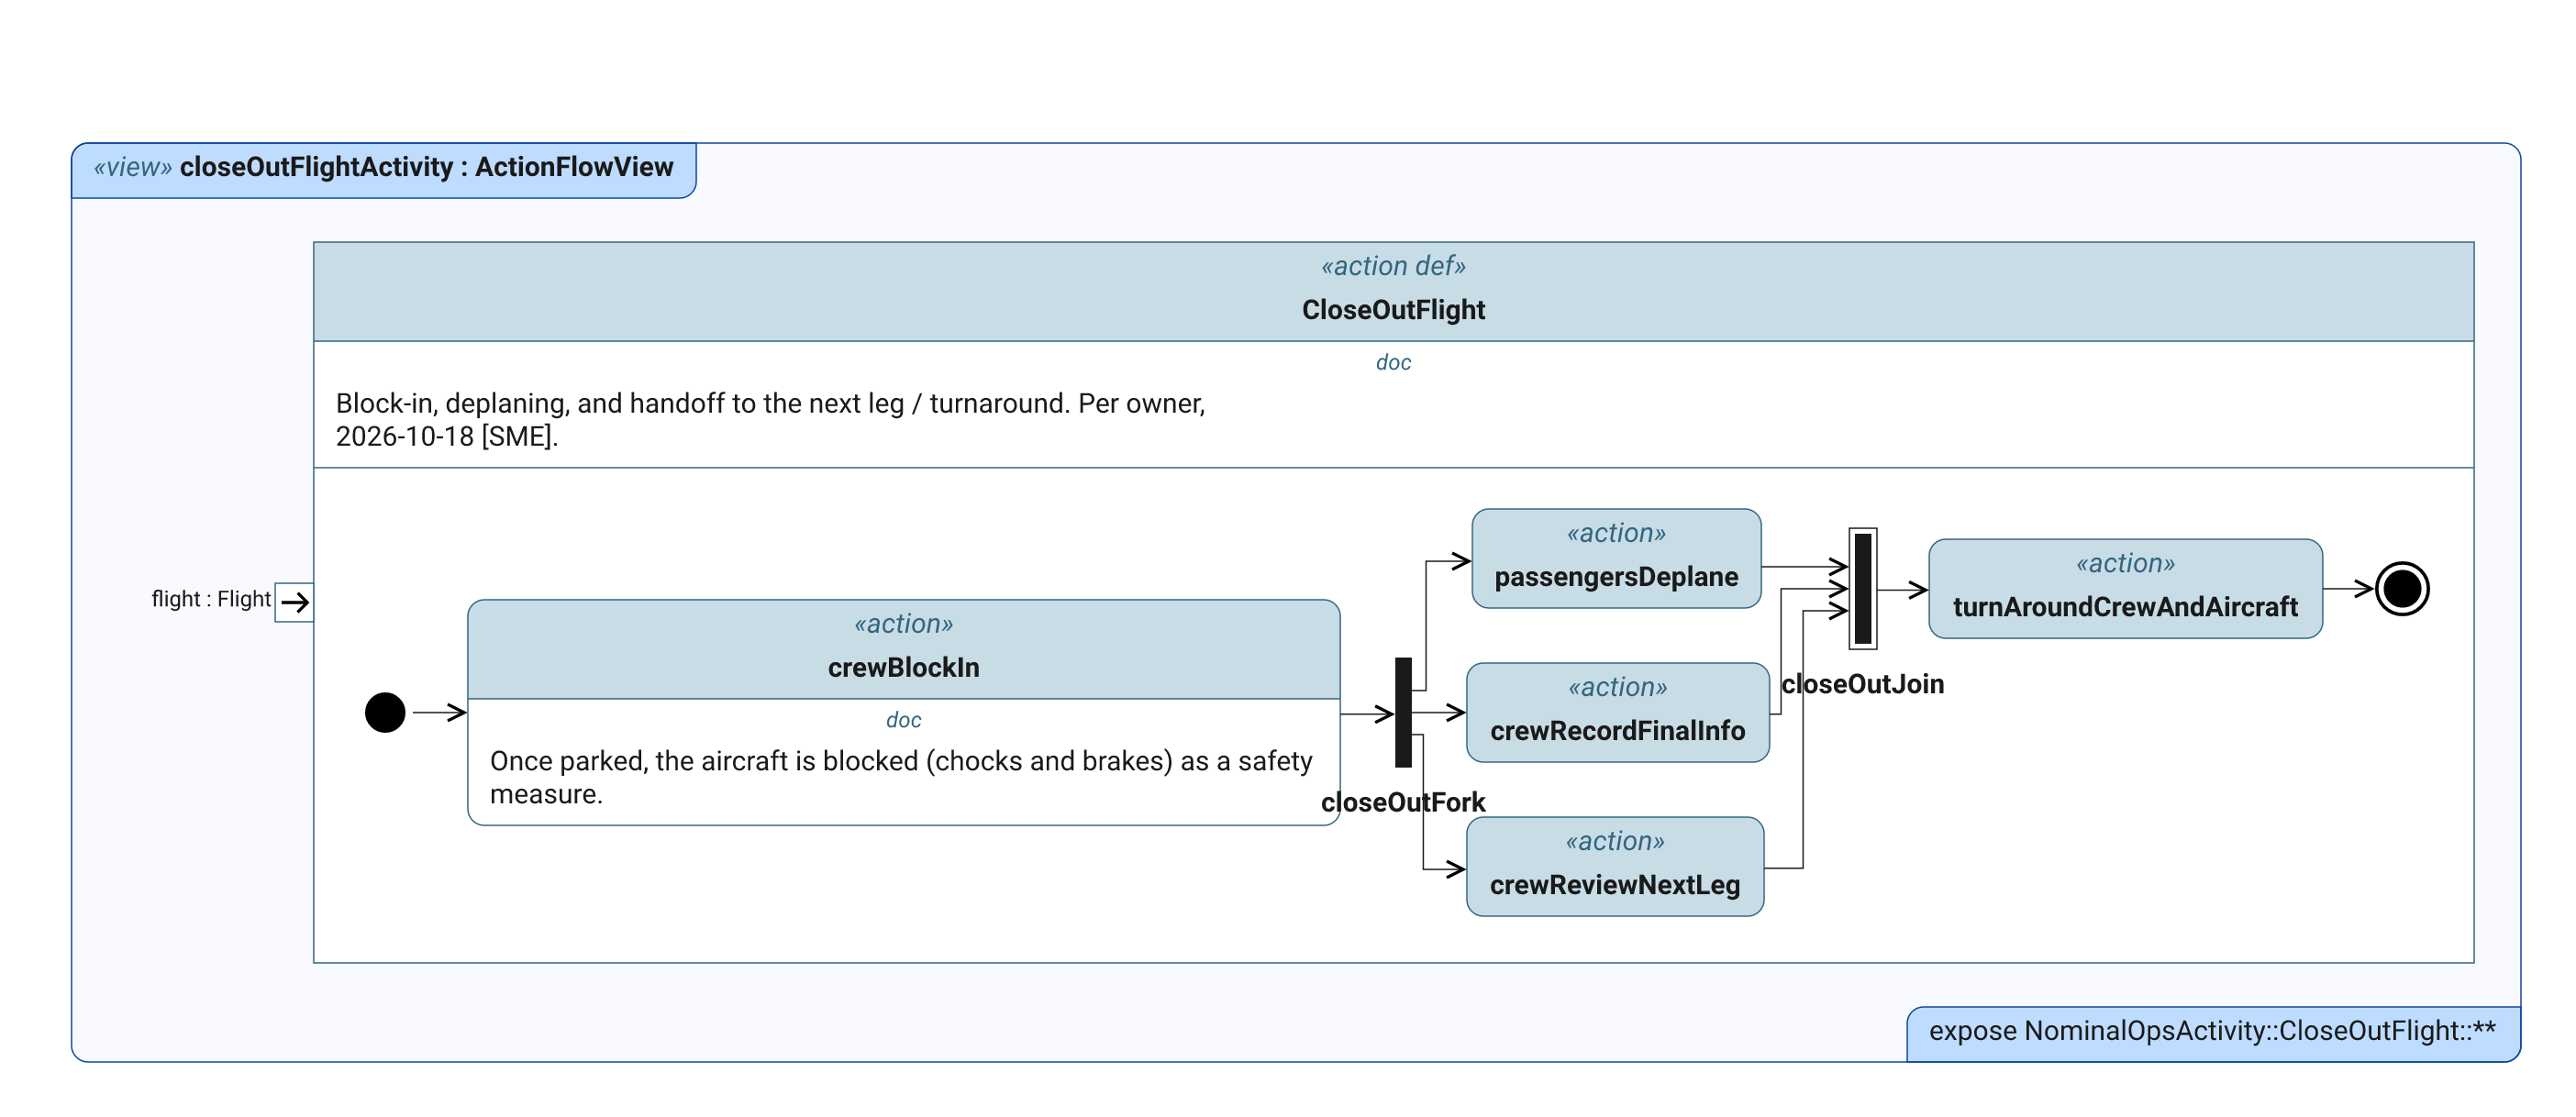
\includegraphics[width=\linewidth,height=0.8\textheight,keepaspectratio]{sysml/diagram-closeOutFlightActivity}
\caption{Nominal operations, Close Out Flight: block-in, deplaning and turnaround. View \texttt{closeOutFlightActivity}; source \texttt{nas\_activity\_diagram-nominal\_ops.sysml}; rendered 2026-10-18.}
\label{fig:sysml-closeOutFlightActivity}
\end{figure}
\end{landscape}


\subsection{Full Stakeholder Register}
\label{app:stakeholders}
\plantodo{S7}{Introduce the two tables below and cite each from the body: the stakeholder assessment (Table~\ref{tab:stakeholder-assessment-excerpt}) and the trace from each stakeholder objective to the requirements (Table~\ref{tab:requirements-objectives}).}

% ---- Generated tables (tools/export_report_tables.py). Do not edit the .tex files in
% figures/tables/: change the stakeholder workbook or the model and rerun the script.
% Owner, 2026-10-22: the whole assessment sheet and the whole objectives sheet go here.
% Generated by tools/export_report_tables.py on 2026-10-22 from knowledge/models/capstone_stakeholder_assessment.xlsx, sheet "Stakeholder Assessment".
% Do not edit: change the source and rerun the script.

\begingroup\footnotesize\setlength{\tabcolsep}{3pt}\setlength{\LTcapwidth}{\textwidth}
\begin{longtable}{@{}>{\raggedright\arraybackslash}p{1.9cm}>{\raggedright\arraybackslash}p{3.3cm}>{\raggedright\arraybackslash}p{3.2cm}>{\raggedright\arraybackslash}p{1.6cm}>{\raggedright\arraybackslash}p{1.6cm}>{\raggedright\arraybackslash}p{0.8cm}>{\raggedright\arraybackslash}p{2.3cm}@{}}
\caption{Stakeholder assessment: all 48 candidate stakeholders, sorted by decision score (\texttt{capstone\_stakeholder\_assessment.xlsx}). Score is standalone importance (high 3, medium 2, low 1) plus trajectory-decision impact (yes 2, indirect 1, no 0); the workbook's other columns (MOPs, MOEs, rationale) are not shown.}\label{tab:stakeholder-assessment-excerpt}\\
\toprule
\textbf{PESTLE domain} & \textbf{Stakeholder} & \textbf{Stated interest} & \textbf{Trajectory impact} & \textbf{Importance} & \textbf{Score} & \textbf{Recommended treatment} \\
\midrule
\endfirsthead
\multicolumn{7}{@{}l}{\textit{Table \thetable{} continued}}\\
\toprule
\textbf{PESTLE domain} & \textbf{Stakeholder} & \textbf{Stated interest} & \textbf{Trajectory impact} & \textbf{Importance} & \textbf{Score} & \textbf{Recommended treatment} \\
\midrule
\endhead
\bottomrule
\endlastfoot
Economic & Adjacent Airspace Users & Throughput and reliability & Yes & High & 5 & Standalone \\
Technical & Air traffic controllers & Predictable aircraft behavior & Yes & High & 5 & Standalone \\
Economic & Airlines & Profitability & Yes & High & 5 & Standalone \\
Economic & Airports & Revenue and capacity & Yes & High & 5 & Standalone \\
Economic & Cargo operators & Throughput and reliability & Yes & High & 5 & Standalone \\
Technical & Dispatchers & Operational optimization & Yes & High & 5 & Standalone \\
Political & Militaries & Navigable airspace \& resources with priority & Yes & High & 5 & Standalone \\
Economic & Engine manufacturers & Product performance and aftermarket revenue & Indirect & High & 4 & Consider /\allowbreak{} Consolidate \\
Social & Flight crews & Workload and quality of life & Indirect & High & 4 & Consider /\allowbreak{} Consolidate \\
Social & Local communities & Noise and environmental impacts & Indirect & High & 4 & Consider /\allowbreak{} Consolidate \\
Environmental & Local communities & Reduced noise & Indirect & High & 4 & Consider /\allowbreak{} Consolidate \\
Social & Business travelers & Schedule reliability & Indirect & Medium & 3 & Consider /\allowbreak{} Consolidate \\
Environmental & Environmental advocacy groups & Reduced emissions & Indirect & Medium & 3 & Consider /\allowbreak{} Consolidate \\
Political & Federal Aviation Administration & Safe and efficient airspace & No & High & 3 & Consider /\allowbreak{} Consolidate \\
Political & ICAO & International standards & Indirect & Medium & 3 & Consider /\allowbreak{} Consolidate \\
Economic & Labor unions & Compensation and job security & Indirect & Medium & 3 & Consider /\allowbreak{} Consolidate \\
Technical & Maintenance personnel & Maintainability & Indirect & Medium & 3 & Consider /\allowbreak{} Consolidate \\
Economic & Passengers & Affordable travel & No & High & 3 & Consider /\allowbreak{} Consolidate \\
Economic & Aircraft manufacturers & Product competitiveness & Indirect & Low & 2 & Boundary input /\allowbreak{} omit \\
Environmental & Airport authorities & Sustainable operations & Indirect & Low & 2 & Boundary input /\allowbreak{} omit \\
Technical & Avionics suppliers & System integration & Indirect & Low & 2 & Boundary input /\allowbreak{} omit \\
Social & Cabin crews & Safety and operational effectiveness & Indirect & Low & 2 & Boundary input /\allowbreak{} omit \\
Legal & Certification authorities & Regulatory compliance & No & Medium & 2 & Boundary input /\allowbreak{} omit \\
Environmental & Climate organizations & Decarbonization & Indirect & Low & 2 & Boundary input /\allowbreak{} omit \\
Social & Families of passengers & Safety & Indirect & Low & 2 & Boundary input /\allowbreak{} omit \\
Environmental & Governments & Emissions targets & Indirect & Low & 2 & Boundary input /\allowbreak{} omit \\
Economic & Insurers & Risk reduction & Indirect & Low & 2 & Boundary input /\allowbreak{} omit \\
Legal & International treaty organizations & Harmonization of standards & Indirect & Low & 2 & Boundary input /\allowbreak{} omit \\
Economic & Investors and shareholders & Return on investment & Indirect & Low & 2 & Boundary input /\allowbreak{} omit \\
Legal & Labor regulators & Worker protections & Indirect & Low & 2 & Boundary input /\allowbreak{} omit \\
Economic & Lessors & Return conditions & Indirect & Low & 2 & Boundary input /\allowbreak{} omit \\
Social & Passengers & Safety and convenience & Indirect & Low & 2 & Boundary input /\allowbreak{} omit \\
Political & State and local governments & Airports, jobs, and noise concerns & No & Medium & 2 & Boundary input /\allowbreak{} omit \\
Social & Tourism industry & Mobility and economic activity & Indirect & Low & 2 & Boundary input /\allowbreak{} omit \\
Technical & Aircraft systems engineers & System performance & No & Low & 1 & Boundary input /\allowbreak{} omit \\
Legal & Aviation lawyers & Compliance and risk & No & Low & 1 & Boundary input /\allowbreak{} omit \\
Technical & Certification engineers & Verification evidence & No & Low & 1 & Boundary input /\allowbreak{} omit \\
Political & Congress and legislatures & Economic growth and public accountability & No & Low & 1 & Boundary input /\allowbreak{} omit \\
Legal & Courts & Liability resolution & No & Low & 1 & Boundary input /\allowbreak{} omit \\
Political & Department of Defense & National security and airspace access & No & Low & 1 & Boundary input /\allowbreak{} omit \\
Political & Department of Transportation & National transportation policy & No & Low & 1 & Boundary input /\allowbreak{} omit \\
Economic & Fuel suppliers & Fuel demand & No & Low & 1 & Boundary input /\allowbreak{} omit \\
Environmental & Future generations (societal proxy) & Long-term sustainability & No & Low & 1 & Boundary input /\allowbreak{} omit \\
Political & National Transportation Safety Board & Prevent accidents & No & Low & 1 & Boundary input /\allowbreak{} omit \\
Legal & Privacy regulators & Passenger data protection & No & Low & 1 & Boundary input /\allowbreak{} omit \\
Technical & Researchers and universities & Innovation & No & Low & 1 & Boundary input /\allowbreak{} omit \\
Technical & Software developers & Correct implementation & No & Low & 1 & Boundary input /\allowbreak{} omit \\
Social & Trainers \& Educators & Regulatory stability \& standard definitions & No & Low & 1 & Boundary input /\allowbreak{} omit \\
\end{longtable}
\endgroup


\begin{landscape}
% Generated by tools/export_report_tables.py on 2026-10-22 from knowledge/models/stakeholder-objective-ontology.md and cameo_models/requirements_*.sysml.
% Do not edit: change the source and rerun the script.

\begingroup\footnotesize\setlength{\tabcolsep}{3pt}\setlength{\LTcapwidth}{\textwidth}
\begin{longtable}{@{}>{\raggedright\arraybackslash}p{3.0cm}>{\raggedright\arraybackslash}p{1.8cm}>{\raggedright\arraybackslash}p{2.4cm}>{\raggedright\arraybackslash}p{2.6cm}>{\raggedright\arraybackslash}p{5.1cm}>{\raggedright\arraybackslash}p{6.4cm}@{}}
\caption{Stakeholder objectives traced to requirements: each of the 43 objective rows of the stakeholder objective ontology, the stakeholder requirements that serve it (an airline requirement can serve another stakeholder's objective), and the system requirements and HLRs reached through those that are in the study or held as background.}\label{tab:requirements-objectives}\\
\toprule
\textbf{Objective} & \textbf{Trajectory impact} & \textbf{Stakeholder req.\ in the study} & \textbf{Background or out of study} & \textbf{System req.\ reached (in the study)} & \textbf{HLRs reached} \\
\midrule
\endfirsthead
\multicolumn{6}{@{}l}{\textit{Table \thetable{} continued}}\\
\toprule
\textbf{Objective} & \textbf{Trajectory impact} & \textbf{Stakeholder req.\ in the study} & \textbf{Background or out of study} & \textbf{System req.\ reached (in the study)} & \textbf{HLRs reached} \\
\midrule
\endhead
\bottomrule
\endlastfoot
\multicolumn{6}{@{}l}{\textbf{Airline}}\\*
Fuel cost & Yes & SN-AIR-01, SN-AIR-05 &  & SLR-PLN-01, SLR-PLN-02, SLR-CLR-09, SLR-CLR-13, SLR-INF-02, SLR-EXE-03, SLR-MEA-02 & HLR-CRW-03, HLR-CRW-05, HLR-OPS-01, HLR-OPS-05, HLR-OPS-07, HLR-ATC-05, HLR-ATC-07, HLR-ATC-08, HLR-ACF-01, HLR-ACF-05 \\
Crew cost & Indirect & SN-AIR-01 &  & SLR-PLN-01, SLR-PLN-02, SLR-CLR-09, SLR-EXE-03, SLR-MEA-02 & HLR-CRW-03, HLR-CRW-05, HLR-OPS-01, HLR-OPS-07, HLR-ATC-07, HLR-ACF-01, HLR-ACF-05 \\
Aircraft utilization & Indirect & SN-AIR-02 &  & SLR-INF-07, SLR-APT-04 & HLR-CRW-04, HLR-OPS-06, HLR-APT-01, HLR-APT-02 \\
Maintenance & Indirect & SN-AIR-01 &  & SLR-PLN-01, SLR-PLN-02, SLR-CLR-09, SLR-EXE-03, SLR-MEA-02 & HLR-CRW-03, HLR-CRW-05, HLR-OPS-01, HLR-OPS-07, HLR-ATC-07, HLR-ACF-01, HLR-ACF-05 \\
Schedule integrity & Yes & SN-AIR-02, SN-AIR-03, SN-AIR-05 &  & SLR-CLR-04, SLR-CLR-13, SLR-INF-02, SLR-INF-07, SLR-APT-04 & HLR-CRW-04, HLR-OPS-05, HLR-OPS-06, HLR-ATC-05, HLR-ATC-08, HLR-ACF-04, HLR-ACF-05, HLR-APT-01, HLR-APT-02 \\
Passenger connections & Yes & SN-AIR-02, SN-AIR-05 & SN-AIR-04 (out of study) & SLR-CLR-13, SLR-INF-02, SLR-INF-07, SLR-APT-04 & HLR-CRW-04, HLR-OPS-05, HLR-OPS-06, HLR-ATC-05, HLR-ATC-08, HLR-ACF-05, HLR-APT-01, HLR-APT-02 \\
Delay cost & Yes & SN-AIR-01, SN-AIR-03 & SN-AIR-04 (out of study) & SLR-PLN-01, SLR-PLN-02, SLR-CLR-04, SLR-CLR-09, SLR-INF-07, SLR-EXE-03, SLR-MEA-02 & HLR-CRW-03, HLR-CRW-04, HLR-CRW-05, HLR-OPS-01, HLR-OPS-06, HLR-OPS-07, HLR-ATC-07, HLR-ACF-01, HLR-ACF-04, HLR-ACF-05 \\
Revenue & Indirect & SN-AIR-01 &  & SLR-PLN-01, SLR-PLN-02, SLR-CLR-09, SLR-EXE-03, SLR-MEA-02 & HLR-CRW-03, HLR-CRW-05, HLR-OPS-01, HLR-OPS-07, HLR-ATC-07, HLR-ACF-01, HLR-ACF-05 \\
Dispatch reliability & Indirect & SN-AIR-02 &  & SLR-INF-07, SLR-APT-04 & HLR-CRW-04, HLR-OPS-06, HLR-APT-01, HLR-APT-02 \\
Flight Safety & Yes & SN-ATC-01 & SN-PAX-01 (out of study) & SLR-PLN-06, SLR-CLR-01, SLR-CLR-02, SLR-INF-01, SLR-EXE-02 & HLR-CRW-01, HLR-OPS-02, HLR-ATC-01, HLR-ATC-02, HLR-ATC-03, HLR-ATC-04, HLR-ACF-02, HLR-ACF-06 \\
\midrule
\multicolumn{6}{@{}l}{\textbf{Passenger}}\\*
Ticket price & No & SN-AIR-01 &  & SLR-PLN-01, SLR-PLN-02, SLR-CLR-09, SLR-EXE-03, SLR-MEA-02 & HLR-CRW-03, HLR-CRW-05, HLR-OPS-01, HLR-OPS-07, HLR-ATC-07, HLR-ACF-01, HLR-ACF-05 \\
Travel time & Yes & SN-AIR-02 & SN-PAX-02 (out of study) & SLR-INF-07, SLR-APT-04 & HLR-CRW-04, HLR-OPS-06, HLR-APT-01, HLR-APT-02 \\
Connection reliability & Yes & SN-AIR-02 & SN-PAX-02 (out of study) & SLR-INF-07, SLR-APT-04 & HLR-CRW-04, HLR-OPS-06, HLR-APT-01, HLR-APT-02 \\
Schedule convenience & Indirect & SN-AIR-01 &  & SLR-PLN-01, SLR-PLN-02, SLR-CLR-09, SLR-EXE-03, SLR-MEA-02 & HLR-CRW-03, HLR-CRW-05, HLR-OPS-01, HLR-OPS-07, HLR-ATC-07, HLR-ACF-01, HLR-ACF-05 \\
Comfort & Yes & SN-AIR-01 & SN-PAX-03 (out of study) & SLR-PLN-01, SLR-PLN-02, SLR-CLR-09, SLR-EXE-03, SLR-MEA-02 & HLR-CRW-03, HLR-CRW-05, HLR-OPS-01, HLR-OPS-07, HLR-ATC-07, HLR-ACF-01, HLR-ACF-05 \\
Disruption risk & Indirect & SN-AIR-02 & SN-PAX-02 (out of study) & SLR-INF-07, SLR-APT-04 & HLR-CRW-04, HLR-OPS-06, HLR-APT-01, HLR-APT-02 \\
\midrule
\multicolumn{6}{@{}l}{\textbf{ATC /\allowbreak{} ANSP}}\\*
Safety/\allowbreak{}separation & Yes & SN-ATC-01 &  & SLR-PLN-06, SLR-CLR-01, SLR-CLR-02, SLR-INF-01, SLR-EXE-02 & HLR-CRW-01, HLR-OPS-02, HLR-ATC-01, HLR-ATC-02, HLR-ATC-03, HLR-ATC-04, HLR-ACF-02, HLR-ACF-06 \\
Sector workload & Yes & SN-ATC-04 &  & SLR-CLR-15 & HLR-ATC-06 \\
Capacity & Yes & SN-ATC-02 &  & SLR-PLN-06 & HLR-OPS-02 \\
Predictability & Yes & SN-AIR-02 & SN-ATC-03 (out of study) & SLR-INF-07, SLR-APT-04 & HLR-CRW-04, HLR-OPS-06, HLR-APT-01, HLR-APT-02 \\
Delay (ATC-attributed) & Yes & SN-AIR-02 & SN-ATC-05 (out of study) & SLR-INF-07, SLR-APT-04 & HLR-CRW-04, HLR-OPS-06, HLR-APT-01, HLR-APT-02 \\
Traffic complexity & Yes & SN-ATC-04 &  & SLR-CLR-15 & HLR-ATC-06 \\
\midrule
\multicolumn{6}{@{}l}{\textbf{Airport}}\\*
Gate utilization & Indirect & SN-AIR-02 & SN-APT-01 (out of study) & SLR-INF-07, SLR-APT-04 & HLR-CRW-04, HLR-OPS-06, HLR-APT-01, HLR-APT-02 \\
Runway utilization & Yes & SN-AIR-02 & SN-APT-02 (out of study) & SLR-INF-07, SLR-APT-04 & HLR-CRW-04, HLR-OPS-06, HLR-APT-01, HLR-APT-02 \\
Surface congestion & Yes & SN-AIR-02 & SN-APT-03 (out of study) & SLR-INF-07, SLR-APT-04 & HLR-CRW-04, HLR-OPS-06, HLR-APT-01, HLR-APT-02 \\
Turnaround performance & Indirect & SN-AIR-02 & SN-APT-01 (out of study) & SLR-INF-07, SLR-APT-04 & HLR-CRW-04, HLR-OPS-06, HLR-APT-01, HLR-APT-02 \\
Passenger throughput & No & SN-AIR-02 & SN-APT-01 (out of study) & SLR-INF-07, SLR-APT-04 & HLR-CRW-04, HLR-OPS-06, HLR-APT-01, HLR-APT-02 \\
\midrule
\multicolumn{6}{@{}l}{\textbf{Flight Crew}}\\*
Safety & Yes & SN-CRW-03, SN-CRW-06, SN-CRW-07 & SN-CRW-01 (out of study), SN-CRW-02 (out of study) & SLR-PLN-07, SLR-CLR-01, SLR-CLR-02, SLR-CLR-10, SLR-INF-02, SLR-EXE-03, SLR-EXE-06 & HLR-CRW-02, HLR-CRW-03, HLR-CRW-04, HLR-CRW-05, HLR-OPS-03, HLR-OPS-05, HLR-OPS-06, HLR-ATC-01, HLR-ATC-02, HLR-ATC-04, HLR-ATC-08, HLR-ACF-01, HLR-ACF-03, HLR-ACF-05, HLR-ACF-06, HLR-APT-02 \\
Workload & Yes & SN-CRW-03, SN-CRW-08 &  & SLR-CLR-04, SLR-CLR-10, SLR-INF-02, SLR-EXE-03, SLR-EXE-06 & HLR-CRW-02, HLR-CRW-03, HLR-CRW-04, HLR-CRW-05, HLR-OPS-05, HLR-OPS-06, HLR-ATC-04, HLR-ATC-08, HLR-ACF-01, HLR-ACF-03, HLR-ACF-04, HLR-ACF-05 \\
Procedural compliance & Yes & SN-CRW-07, SN-CRW-08 & SN-CRW-02 (out of study) & SLR-PLN-07, SLR-CLR-04 & HLR-CRW-04, HLR-CRW-05, HLR-OPS-03, HLR-OPS-06, HLR-ACF-04, HLR-APT-02 \\
Schedule/\allowbreak{}duty constraints & Indirect & SN-AIR-02 & SN-CRW-05 (out of study) & SLR-INF-07, SLR-APT-04 & HLR-CRW-04, HLR-OPS-06, HLR-APT-01, HLR-APT-02 \\
Operational flexibility & Yes & SN-AIR-01, SN-AIR-05 & SN-CRW-01 (out of study), SN-CRW-04 (out of study) & SLR-PLN-01, SLR-PLN-02, SLR-CLR-09, SLR-CLR-13, SLR-INF-02, SLR-EXE-03, SLR-MEA-02 & HLR-CRW-03, HLR-CRW-05, HLR-OPS-01, HLR-OPS-05, HLR-OPS-07, HLR-ATC-05, HLR-ATC-07, HLR-ATC-08, HLR-ACF-01, HLR-ACF-05 \\
\midrule
\multicolumn{6}{@{}l}{\textbf{Environmental /\allowbreak{} Societal}}\\*
CO\textsubscript{2} & Yes & SN-AIR-01, SN-AIR-05 & SN-ENV-01 (background) & SLR-PLN-01, SLR-PLN-02, SLR-CLR-09, SLR-CLR-13, SLR-INF-02, SLR-EXE-03, SLR-MEA-02 & HLR-CRW-03, HLR-CRW-05, HLR-OPS-01, HLR-OPS-05, HLR-OPS-07, HLR-ATC-05, HLR-ATC-07, HLR-ATC-08, HLR-ACF-01, HLR-ACF-05 \\
NOx & Yes & SN-AIR-01, SN-AIR-05 & SN-ENV-01 (background) & SLR-PLN-01, SLR-PLN-02, SLR-CLR-09, SLR-CLR-13, SLR-INF-02, SLR-EXE-03, SLR-MEA-02 & HLR-CRW-03, HLR-CRW-05, HLR-OPS-01, HLR-OPS-05, HLR-OPS-07, HLR-ATC-05, HLR-ATC-07, HLR-ATC-08, HLR-ACF-01, HLR-ACF-05 \\
Contrail/\allowbreak{}climate effects & Yes & SN-AIR-01, SN-AIR-05 & SN-ENV-01 (background) & SLR-PLN-01, SLR-PLN-02, SLR-CLR-09, SLR-CLR-13, SLR-INF-02, SLR-EXE-03, SLR-MEA-02 & HLR-CRW-03, HLR-CRW-05, HLR-OPS-01, HLR-OPS-05, HLR-OPS-07, HLR-ATC-05, HLR-ATC-07, HLR-ATC-08, HLR-ACF-01, HLR-ACF-05 \\
Noise & Yes & SN-AIR-01, SN-AIR-05 & SN-ENV-02 (out of study) & SLR-PLN-01, SLR-PLN-02, SLR-CLR-09, SLR-CLR-13, SLR-INF-02, SLR-EXE-03, SLR-MEA-02 & HLR-CRW-03, HLR-CRW-05, HLR-OPS-01, HLR-OPS-05, HLR-OPS-07, HLR-ATC-05, HLR-ATC-07, HLR-ATC-08, HLR-ACF-01, HLR-ACF-05 \\
Local air quality & Indirect & SN-AIR-01, SN-AIR-05 & SN-ENV-01 (background) & SLR-PLN-01, SLR-PLN-02, SLR-CLR-09, SLR-CLR-13, SLR-INF-02, SLR-EXE-03, SLR-MEA-02 & HLR-CRW-03, HLR-CRW-05, HLR-OPS-01, HLR-OPS-05, HLR-OPS-07, HLR-ATC-05, HLR-ATC-07, HLR-ATC-08, HLR-ACF-01, HLR-ACF-05 \\
\midrule
\multicolumn{6}{@{}l}{\textbf{Military}}\\*
Mission effectiveness & Yes &  & \textit{none} &  &  \\
Mission timing & Yes &  & \textit{none} &  &  \\
Fuel availability & Indirect &  & \textit{none} &  &  \\
Airspace access & Yes &  & SN-MIL-01 (out of study) &  &  \\
Operational security & No &  & \textit{none} &  &  \\
Resilience & Indirect &  & \textit{none} &  &  \\
\midrule
\multicolumn{6}{@{}l}{\textbf{Stakeholder requirements that name no objective row}}\\*
\textit{Airline} & &  & SN-AIR-06 (out of study) & & \\
\textit{Regulator} & &  & SN-GOV-01 (background) & & \\
\textit{Regulator} & &  & SN-GOV-02 (out of study) & & \\
\end{longtable}
\endgroup

\end{landscape}
% ---- end generated tables
\FloatBarrier

\subsection{Requirements Decomposition}
\label{app:requirements}
\plantodo{S7, S10}{Introduce the decomposition (Table~\ref{tab:requirements-decomposition}) and cite it from the body: how to read it, why out-of-study requirements stop at the system tier (D-031), and where the studied thread runs (SN-AIR-05 $\rightarrow$ SLR-INF-02 / SLR-CLR-13).}

% ---- Generated table (tools/export_report_tables.py): the Decomposition sheet of
% cameo_models/print/requirements-review.xlsx in full. Owner, 2026-10-22.
\begin{landscape}
% Generated by tools/export_report_tables.py on 2026-10-22 from projects/nas-sos-capstone/cameo_models/requirements_*.sysml.
% Do not edit: change the source and rerun the script.

\begingroup\footnotesize\setlength{\tabcolsep}{4pt}\setlength{\LTcapwidth}{\textwidth}
\begin{longtable}{@{}>{\raggedright\arraybackslash}p{6.4cm}>{\raggedright\arraybackslash}p{7.2cm}>{\raggedright\arraybackslash}p{8.6cm}@{}}
\caption{Requirements decomposition: each stakeholder requirement, the system requirements that answer it, and the sub-system requirements (HLRs) that come from each. 30 stakeholder requirements, 42 system requirements (23 in the study) and 29 HLRs, from the SysML v2 model. A requirement's text is given where it first appears; later appearances give its ID. Grey: out of study, with no HLR, the study's cut being made at the HLR tier. \textsc{[background]}: held fixed as an input. \textsc{[improved]}: not done by today's NAS. \textsc{[goal]}: written with ``should''.}\label{tab:requirements-decomposition}\\
\toprule
\textbf{Stakeholder requirement} & \textbf{System requirement (the NAS shall)} & \textbf{Sub-system requirement (HLR)} \\
\midrule
\endfirsthead
\multicolumn{3}{@{}l}{\textit{Table \thetable{} continued}}\\
\toprule
\textbf{Stakeholder requirement} & \textbf{System requirement (the NAS shall)} & \textbf{Sub-system requirement (HLR)} \\
\midrule
\endhead
\bottomrule
\endlastfoot
\multicolumn{3}{@{}l}{\textbf{Stakeholder: Airline}}\\*
\textbf{SN-AIR-01} The NAS shall provide a means for the airline to plan and fly each flight on the route, altitude and speed it chooses. & \textbf{SLR-PLN-01} The NAS shall produce for each scheduled flight a flight plan that states its route, cruise altitude, cruise speed and fuel load. \textit{(also SN-CRW-02)} & \textbf{HLR-OPS-01} Flight operations shall plan each flight's route, cruise altitude, cruise speed and fuel load from a model of the performance of the aircraft assigned to it, with the fuel reserve the operating rules require. \textit{(also SLR-PLN-02, SLR-PLN-04)} \\
\cmidrule(l){2-3}
 & \textbf{SLR-PLN-02} The NAS shall compute each flight plan from the performance of the aircraft assigned to the flight. & \textbf{HLR-OPS-01} \textit{(text above)} \\
\cmidrule(l){2-3}
 & \textbf{SLR-CLR-09} The NAS shall answer each flight crew request for a route, altitude or speed change with an approval, an amended clearance or a refusal. \textit{(also SN-CRW-04, SN-PAX-03)} & \textbf{HLR-CRW-03} The flight crew shall ask air traffic control for a change of route, altitude or speed when the crew deems it beneficial, optionally in collaboration with the dispatcher. \textit{(also SLR-EXE-03)} \\
 &  & \textbf{HLR-ATC-07} Air traffic control shall answer each flight crew request for a route, altitude or speed change with an approval, an amended clearance or 'unable'. \\
\cmidrule(l){2-3}
 & \textbf{SLR-EXE-03} The NAS shall predict each flight's arrival time, fuel at destination, optimum altitude and maximum altitude from the aircraft's estimated performance. \textit{(also SN-CRW-03)} & \textbf{HLR-CRW-03} \textit{(text above)} \\
 &  & \textbf{HLR-CRW-05} The flight crew shall enter the load sheet weights and the released cost index into the flight management system before departure. \textit{(also SLR-PLN-07)} \\
 &  & \textbf{HLR-ACF-01} The flight management system shall predict the flight's arrival time, fuel at the destination, optimum altitude and maximum altitude from the entered weights, the cost index and the forecast winds. \\
 &  & \textbf{HLR-ACF-05} The flight management system shall make its current gross weight and its predicted optimum and maximum altitudes available for sharing with the party that decides, whether through the airline's systems or air traffic control's. \textit{(also SLR-INF-02)} \\
\cmidrule(l){2-3}
 & \textbf{SLR-MEA-02} The NAS shall report the fuel burned and the CO\textsubscript{2} emitted by each flight, at 3.16 kg of CO\textsubscript{2} per kg of fuel. \textit{(also SN-ENV-01)} & \textbf{HLR-OPS-07} Flight operations shall report each flight's fuel burned and its CO\textsubscript{2} emitted at 3.16 kg of CO\textsubscript{2} per kg of fuel. \\
\cmidrule(l){1-3}
\textbf{SN-AIR-02} The NAS shall provide a means for each flight to achieve arrival at its destination gate at its scheduled arrival time. & \textbf{SLR-INF-07} The NAS shall send the airline and the destination airport an updated arrival estimate whenever a flight's estimate changes by more than 5 minutes. \textit{(also SN-AIR-03, SN-APT-01)} & \textbf{HLR-CRW-04} The flight crew shall tell the dispatcher of each change to the cleared trajectory. \textit{(also SLR-EXE-06, SLR-CLR-04)} \\
 &  & \textbf{HLR-OPS-06} The dispatcher shall re-plan the flight with its crew when a trajectory change puts the arrival time, the fuel at the destination or flight safety at risk. \textit{(also SLR-CLR-04, SLR-EXE-06)} \\
\cmidrule(l){2-3}
 & \textcolor{gray}{\textbf{SLR-APT-01} \textsc{[out of study]} The NAS shall assign each arriving flight a gate before it lands. \textit{(also SN-APT-01)}} & \textcolor{gray}{\textit{no HLR: not carried into the study}} \\
\cmidrule(l){2-3}
 & \textbf{SLR-APT-04} The NAS shall have each aircraft fuelled, loaded and sealed by its scheduled off- block time. & \textbf{HLR-APT-01} Airport operations shall have each aircraft fuelled, loaded and sealed by its scheduled off-block time. \\
 &  & \textbf{HLR-APT-02} Airport operations shall report the fuel uplifted and the load put on board to the flight crew and the load planner before off-block. \textit{(also SLR-PLN-07)} \\
\cmidrule(l){2-3}
 & \textcolor{gray}{\textbf{SLR-MEA-03} \textsc{[out of study]} The NAS shall report each flight's gate arrival time against its scheduled arrival time. \textit{(also SN-PAX-02)}} & \textcolor{gray}{\textit{no HLR: not carried into the study}} \\
\cmidrule(l){1-3}
\textbf{SN-AIR-03} The NAS shall inform the airline of airspace and airport constraints that will delay or reroute its flights early enough for the airline to re-plan. & \textcolor{gray}{\textbf{SLR-FLW-07} \textsc{[out of study]} The NAS shall give traffic flow managers and airlines the activation schedule of special use airspace before the affected flight plans are filed. \textit{(also SN-MIL-01)}} & \textcolor{gray}{\textit{no HLR: not carried into the study}} \\
\cmidrule(l){2-3}
 & \textbf{SLR-CLR-04} The NAS shall provide a two-way communication path from the flight crew to the controlling facility and to the dispatcher for the whole flight. \textit{(also SN-CRW-08)} & \textbf{HLR-CRW-04} \textit{(text above)} \\
 &  & \textbf{HLR-OPS-06} \textit{(text above)} \\
 &  & \textbf{HLR-ACF-04} The aircraft communication system shall carry voice and data between the flight crew and both air traffic control and the dispatcher for the whole flight. \\
\cmidrule(l){2-3}
 & \textbf{SLR-INF-07} \textit{(text above)} & \textbf{HLR-CRW-04} \textit{(text above)} \\
 &  & \textbf{HLR-OPS-06} \textit{(text above)} \\
\cmidrule(l){1-3}
\textcolor{gray}{\textbf{SN-AIR-04} \textsc{[out of study]} The NAS shall let the airline choose which of its own flights takes a delay that the airline has been assigned.} & \textcolor{gray}{\textbf{SLR-FLW-04} \textsc{[out of study]} The NAS shall let an airline exchange its own flights among the departure slots it has been assigned.} & \textcolor{gray}{\textit{no HLR: not carried into the study}} \\
\cmidrule(l){1-3}
\textbf{SN-AIR-05} The NAS shall take the airline's priorities for a flight (fuel against time, and protected connections) into account when a change to that flight's trajectory is required. & \textbf{SLR-CLR-13} \textsc{[goal, improved]} The NAS should choose, among the maneuvers that restore separation, the one with the lowest impact on the aircraft involved. \textit{(also SN-ENV-01)} & \textbf{HLR-ATC-05} \textsc{[goal, improved]} Air traffic control should choose, among the clearances that resolve a conflict and can be flown, the one with the lowest impact on the systems involved. \\
\cmidrule(l){2-3}
 & \textbf{SLR-INF-02} \textsc{[improved]} The NAS shall give the party that decides a change to an aircraft's trajectory the information needed to preserve safety and pursue optimality. \textit{(also SN-CRW-03)} & \textbf{HLR-OPS-05} \textsc{[improved]} Flight operations shall make each flight's current gross weight, performance model, relative cost of flight time and connection priority available to the party that decides a change to that flight's trajectory. \\
 &  & \textbf{HLR-ATC-08} \textsc{[improved]} ATC decision support shall use the best information available to it about each flight, including the gross weight, performance model, relative cost of flight time and connection priority the airline has shared, to judge which clearances the aircraft can fly and what each costs. \\
 &  & \textbf{HLR-ACF-05} \textit{(text above)} \\
\cmidrule(l){1-3}
\textcolor{gray}{\textbf{SN-AIR-06} \textsc{[out of study]} The NAS shall keep the airline's commercially sensitive flight data (aircraft weight, cost index, connection priorities) private.} & \textcolor{gray}{\textbf{SLR-INF-05} \textsc{[out of study]} The NAS shall disclose an airline's shared weight, cost index and connection priority only to the parties deciding that flight's trajectory.} & \textcolor{gray}{\textit{no HLR: not carried into the study}} \\
\midrule
\multicolumn{3}{@{}l}{\textbf{Stakeholder: Air traffic control}}\\*
\textbf{SN-ATC-01} The NAS shall keep every controlled aircraft separated from every other aircraft by at least the applicable separation minimum. & \textbf{SLR-PLN-06} The NAS shall file each flight plan with air traffic control before the flight departs. \textit{(also SN-ATC-02, SN-ATC-03)} & \textbf{HLR-OPS-02} The dispatcher shall file each flight's plan with air traffic control before departure. \\
\cmidrule(l){2-3}
 & \textbf{SLR-CLR-01} The NAS shall keep each pair of controlled aircraft separated by at least the minimum that JO 7110.65BB sets for the airspace they are in. \textit{(also SN-CRW-06, SN-PAX-01)} & \textbf{HLR-ATC-01} Air traffic control shall keep each pair of aircraft it controls separated by at least the applicable minimum, allowing for each aircraft's permitted deviation from its cleared route, altitude and speed. \textit{(also SLR-EXE-02)} \\
 &  & \textbf{HLR-ATC-04} \textsc{[improved]} Air traffic control shall resolve each predicted conflict with a clearance that every aircraft it moves can fly. \textit{(also SLR-CLR-10)} \\
 &  & \textbf{HLR-ACF-06} The aircraft's surveillance system shall broadcast the aircraft's position, altitude, velocity and identity by ADS-B Out. \textit{(also SLR-CLR-02)} \\
\cmidrule(l){2-3}
 & \textbf{SLR-CLR-02} The NAS shall predict a loss of separation between controlled aircraft before it occurs. \textit{(also SN-CRW-06)} & \textbf{HLR-ATC-02} ATC decision support shall alert the sector controller to each predicted loss of separation before it occurs. \\
 &  & \textbf{HLR-ACF-06} \textit{(text above)} \\
\cmidrule(l){2-3}
 & \textcolor{gray}{\textbf{SLR-CLR-03} \textsc{[out of study]} The NAS shall give the controlling facility the position, altitude and identity of each controlled aircraft. \textit{(also SN-ATC-03)}} & \textcolor{gray}{\textit{no HLR: not carried into the study}} \\
\cmidrule(l){2-3}
 & \textcolor{gray}{\textbf{SLR-CLR-05} \textsc{[out of study]} The NAS shall change a controlled aircraft's cleared route, altitude or speed only by a clearance from the facility that has control of that aircraft. \textit{(also SN-GOV-02)}} & \textcolor{gray}{\textit{no HLR: not carried into the study}} \\
\cmidrule(l){2-3}
 & \textbf{SLR-INF-01} The NAS shall give the sector controller the filed route, requested altitude and requested speed of each aircraft before it enters the sector. \textit{(also SN-ATC-03)} & \textbf{HLR-ATC-03} The en-route center shall inform the sector controller of each aircraft's filed route, requested altitude and requested speed before the aircraft enters the sector. \\
\cmidrule(l){2-3}
 & \textbf{SLR-EXE-02} The NAS shall fly each aircraft along its cleared route and at its cleared altitude and speed within the navigation and altitude tolerances of the airspace. \textit{(also SN-ATC-03)} & \textbf{HLR-CRW-01} The flight crew shall safely control the flight from origin to destination, as cleared by air traffic control with or without negotiation, and in collaboration with flight operations. \textit{(also SLR-CLR-08, SLR-PLN-05)} \\
 &  & \textbf{HLR-ATC-01} \textit{(text above)} \\
 &  & \textbf{HLR-ACF-02} The auto flight control system shall hold the aircraft on its cleared route, altitude and speed within the tolerances of the airspace. \\
\cmidrule(l){1-3}
\textbf{SN-ATC-02} The NAS shall keep the number of aircraft in each sector and at each airport within its declared capacity. & \textbf{SLR-PLN-06} \textit{(text above)} & \textbf{HLR-OPS-02} \textit{(text above)} \\
\cmidrule(l){2-3}
 & \textcolor{gray}{\textbf{SLR-PLN-08} \textsc{[out of study]} The NAS shall plan each flight to comply with the traffic management initiatives and special use airspace activations published for its time of flight. \textit{(also SN-MIL-01)}} & \textcolor{gray}{\textit{no HLR: not carried into the study}} \\
\cmidrule(l){2-3}
 & \textcolor{gray}{\textbf{SLR-FLW-06} \textsc{[out of study]} The NAS shall release each flight that has an expect departure clearance time (EDCT) within the permitted window around that time. \textit{(also SN-ATC-03)}} & \textcolor{gray}{\textit{no HLR: not carried into the study}} \\
\cmidrule(l){2-3}
 & \textcolor{gray}{\textbf{SLR-APT-02} \textsc{[out of study]} The NAS shall sequence arrivals and departures so that each runway is used at its declared capacity whenever demand is at or above that rate. \textit{(also SN-APT-02)}} & \textcolor{gray}{\textit{no HLR: not carried into the study}} \\
\cmidrule(l){1-3}
\textcolor{gray}{\textbf{SN-ATC-03} \textsc{[out of study]} The NAS shall make the path each controlled aircraft will fly known to its controller in advance.} & \textbf{SLR-PLN-06} \textit{(text above)} & \textbf{HLR-OPS-02} \textit{(text above)} \\
\cmidrule(l){2-3}
 & \textcolor{gray}{\textbf{SLR-FLW-06} \textit{(text above)}} & \textcolor{gray}{\textit{no HLR: not carried into the study}} \\
\cmidrule(l){2-3}
 & \textcolor{gray}{\textbf{SLR-CLR-03} \textit{(text above)}} & \textcolor{gray}{\textit{no HLR: not carried into the study}} \\
\cmidrule(l){2-3}
 & \textbf{SLR-INF-01} \textit{(text above)} & \textbf{HLR-ATC-03} \textit{(text above)} \\
\cmidrule(l){2-3}
 & \textcolor{gray}{\textbf{SLR-EXE-01} \textsc{[out of study]} The NAS shall hold each flight's cleared route and altitudes in the flight management system as the path the aircraft's guidance follows.} & \textcolor{gray}{\textit{no HLR: not carried into the study}} \\
\cmidrule(l){2-3}
 & \textbf{SLR-EXE-02} \textit{(text above)} & \textbf{HLR-CRW-01} \textit{(text above)} \\
 &  & \textbf{HLR-ATC-01} \textit{(text above)} \\
 &  & \textbf{HLR-ACF-02} \textit{(text above)} \\
\cmidrule(l){1-3}
\textbf{SN-ATC-04} The NAS shall keep the number of control actions a sector controller must take within what one sector team can sustain. & \textbf{SLR-CLR-15} The NAS shall keep the control instructions needed to resolve a conflict within what the sector team can sustain. & \textbf{HLR-ATC-06} Air traffic control shall resolve each predicted conflict within the number of instructions the sector team can sustain. \\
\cmidrule(l){1-3}
\textcolor{gray}{\textbf{SN-ATC-05} \textsc{[out of study]} The NAS shall share unavoidable delay equitably among airspace users.} & \textcolor{gray}{\textbf{SLR-FLW-05} \textsc{[out of study]} The NAS shall assign the delay created by a traffic management initiative equitably among all airspace users.} & \textcolor{gray}{\textit{no HLR: not carried into the study}} \\
\cmidrule(l){2-3}
 & \textcolor{gray}{\textbf{SLR-MEA-04} \textsc{[out of study]} The NAS shall report the delay each flight received from traffic management initiatives, by airline.} & \textcolor{gray}{\textit{no HLR: not carried into the study}} \\
\midrule
\multicolumn{3}{@{}l}{\textbf{Stakeholder: Flight crew}}\\*
\textcolor{gray}{\textbf{SN-CRW-01} \textsc{[out of study]} The NAS shall preserve the captain's final authority over the safe conduct of the flight.} & \textbf{SLR-PLN-05} The NAS shall release a flight only when the dispatcher and the captain both agree that it can be flown safely as planned. \textit{(also SN-GOV-01, SN-GOV-02)} & \textbf{HLR-CRW-01} \textit{(text above)} \\
 &  & \textbf{HLR-OPS-04} The dispatcher shall release a flight only with the captain's agreement that it can be flown safely as planned. \\
\cmidrule(l){2-3}
 & \textbf{SLR-CLR-08} The NAS shall allow the captain to deviate from a clearance when safety requires it, with air traffic control told as soon as practical. \textit{(also SN-GOV-01, SN-PAX-01)} & \textbf{HLR-CRW-01} \textit{(text above)} \\
\cmidrule(l){2-3}
 & \textcolor{gray}{\textbf{SLR-EXE-04} \textsc{[out of study]} The NAS shall change an aircraft's flown trajectory only through flight deck controls operated by the flight crew. \textit{(also SN-GOV-02)}} & \textcolor{gray}{\textit{no HLR: not carried into the study}} \\
\cmidrule(l){1-3}
\textcolor{gray}{\textbf{SN-CRW-02} \textsc{[out of study]} The NAS shall give the flight crew the information needed for each phase of flight before that phase begins.} & \textbf{SLR-PLN-01} \textit{(text above)} & \textbf{HLR-OPS-01} \textit{(text above)} \\
\cmidrule(l){2-3}
 & \textbf{SLR-PLN-07} The NAS shall deliver the dispatch release, flight plan, weather, notices to airmen (NOTAMs) and load sheet to the flight crew before departure. \textit{(also SN-CRW-07)} & \textbf{HLR-CRW-05} \textit{(text above)} \\
 &  & \textbf{HLR-OPS-03} Flight operations shall give the flight crew the dispatch release, flight plan, weather, notices to airmen (NOTAMs) and load sheet before departure. \\
 &  & \textbf{HLR-APT-02} \textit{(text above)} \\
\cmidrule(l){2-3}
 & \textcolor{gray}{\textbf{SLR-INF-06} \textsc{[out of study]} The NAS shall give the dispatcher and the flight crew the reported and forecast weather and turbulence along the planned route. \textit{(also SN-PAX-03)}} & \textcolor{gray}{\textit{no HLR: not carried into the study}} \\
\cmidrule(l){2-3}
 & \textbf{SLR-EXE-06} The NAS shall alert the flight crew, dispatchers and controllers when the fuel predicted at the destination falls below the required reserve. \textit{(also SN-GOV-01, SN-CRW-03, SN-PAX-01)} & \textbf{HLR-CRW-04} \textit{(text above)} \\
 &  & \textbf{HLR-OPS-06} \textit{(text above)} \\
 &  & \textbf{HLR-ACF-03} The flight management system shall alert the flight crew when the fuel it predicts at the destination falls below the required reserve. \\
\cmidrule(l){1-3}
\textbf{SN-CRW-03} The NAS shall give the flight crew only trajectory clearances and instructions that the aircraft can fly, with enough time to set them up. & \textbf{SLR-CLR-10} \textsc{[improved]} The NAS shall issue only clearances that the aircraft can fly. & \textbf{HLR-CRW-02} The flight crew shall accept a clearance only if the aircraft can fly it, and shall answer 'unable' when it cannot. \\
 &  & \textbf{HLR-ATC-04} \textit{(text above)} \\
\cmidrule(l){2-3}
 & \textbf{SLR-INF-02} \textit{(text above)} & \textbf{HLR-OPS-05} \textit{(text above)} \\
 &  & \textbf{HLR-ATC-08} \textit{(text above)} \\
 &  & \textbf{HLR-ACF-05} \textit{(text above)} \\
\cmidrule(l){2-3}
 & \textbf{SLR-EXE-03} \textit{(text above)} & \textbf{HLR-CRW-03} \textit{(text above)} \\
 &  & \textbf{HLR-CRW-05} \textit{(text above)} \\
 &  & \textbf{HLR-ACF-01} \textit{(text above)} \\
 &  & \textbf{HLR-ACF-05} \textit{(text above)} \\
\cmidrule(l){2-3}
 & \textbf{SLR-EXE-06} \textit{(text above)} & \textbf{HLR-CRW-04} \textit{(text above)} \\
 &  & \textbf{HLR-OPS-06} \textit{(text above)} \\
 &  & \textbf{HLR-ACF-03} \textit{(text above)} \\
\cmidrule(l){1-3}
\textcolor{gray}{\textbf{SN-CRW-04} \textsc{[out of study]} The NAS shall let the flight crew ask for a trajectory change and get an answer.} & \textbf{SLR-CLR-09} \textit{(text above)} & \textbf{HLR-CRW-03} \textit{(text above)} \\
 &  & \textbf{HLR-ATC-07} \textit{(text above)} \\
\cmidrule(l){1-3}
\textcolor{gray}{\textbf{SN-CRW-05} \textsc{[out of study]} The NAS shall keep each flight crew member within flight and duty time limits.} & \textcolor{gray}{\textbf{SLR-PLN-09} \textsc{[out of study]} The NAS shall assign to each flight a crew whose duty period, including forecast delay, stays within the limits of 14 CFR Part 117. \textit{(also SN-GOV-01)}} & \textcolor{gray}{\textit{no HLR: not carried into the study}} \\
\cmidrule(l){1-3}
\textbf{SN-CRW-06} The NAS shall provide the flight crew clearances that account for air traffic. & \textbf{SLR-CLR-01} \textit{(text above)} & \textbf{HLR-ATC-01} \textit{(text above)} \\
 &  & \textbf{HLR-ATC-04} \textit{(text above)} \\
 &  & \textbf{HLR-ACF-06} \textit{(text above)} \\
\cmidrule(l){2-3}
 & \textbf{SLR-CLR-02} \textit{(text above)} & \textbf{HLR-ATC-02} \textit{(text above)} \\
 &  & \textbf{HLR-ACF-06} \textit{(text above)} \\
\cmidrule(l){1-3}
\textbf{SN-CRW-07} The NAS shall inform the flight crew of weather, traffic and other safety considerations. & \textbf{SLR-PLN-07} \textit{(text above)} & \textbf{HLR-CRW-05} \textit{(text above)} \\
 &  & \textbf{HLR-OPS-03} \textit{(text above)} \\
 &  & \textbf{HLR-APT-02} \textit{(text above)} \\
\cmidrule(l){1-3}
\textbf{SN-CRW-08} The NAS shall facilitate control of the aircraft across regional sectors, coordinating controls, clearances and handoffs. & \textbf{SLR-CLR-04} \textit{(text above)} & \textbf{HLR-CRW-04} \textit{(text above)} \\
 &  & \textbf{HLR-OPS-06} \textit{(text above)} \\
 &  & \textbf{HLR-ACF-04} \textit{(text above)} \\
\midrule
\multicolumn{3}{@{}l}{\textbf{Stakeholder: Regulator}}\\*
\textbf{SN-GOV-01} \textsc{[background]} The NAS shall conduct every flight within the operating rules of 14 CFR and the FAA's air traffic orders. & \textbf{SLR-PLN-04} The NAS shall load each flight with fuel to reach its destination, then its most distant alternate, then fly 45 minutes at normal cruise. \textit{(also SN-PAX-01)} & \textbf{HLR-OPS-01} \textit{(text above)} \\
\cmidrule(l){2-3}
 & \textbf{SLR-PLN-05} \textit{(text above)} & \textbf{HLR-CRW-01} \textit{(text above)} \\
 &  & \textbf{HLR-OPS-04} \textit{(text above)} \\
\cmidrule(l){2-3}
 & \textcolor{gray}{\textbf{SLR-PLN-09} \textit{(text above)}} & \textcolor{gray}{\textit{no HLR: not carried into the study}} \\
\cmidrule(l){2-3}
 & \textbf{SLR-CLR-08} \textit{(text above)} & \textbf{HLR-CRW-01} \textit{(text above)} \\
\cmidrule(l){2-3}
 & \textbf{SLR-EXE-06} \textit{(text above)} & \textbf{HLR-CRW-04} \textit{(text above)} \\
 &  & \textbf{HLR-OPS-06} \textit{(text above)} \\
 &  & \textbf{HLR-ACF-03} \textit{(text above)} \\
\cmidrule(l){2-3}
 & \textbf{SLR-MEA-01} The NAS shall record each change to an aircraft's trajectory, to its clearance, or to the constraints imposed on it, with the authority that issued it and the time. \textit{(also SN-GOV-02)} & \textbf{HLR-ATC-09} Air traffic control shall record each clearance it issues with the issuing facility and the time. \\
\cmidrule(l){1-3}
\textcolor{gray}{\textbf{SN-GOV-02} \textsc{[out of study]} The NAS shall make one identified authority accountable for each decision that changes a flight's trajectory.} & \textbf{SLR-PLN-05} \textit{(text above)} & \textbf{HLR-CRW-01} \textit{(text above)} \\
 &  & \textbf{HLR-OPS-04} \textit{(text above)} \\
\cmidrule(l){2-3}
 & \textcolor{gray}{\textbf{SLR-CLR-05} \textit{(text above)}} & \textcolor{gray}{\textit{no HLR: not carried into the study}} \\
\cmidrule(l){2-3}
 & \textcolor{gray}{\textbf{SLR-EXE-04} \textit{(text above)}} & \textcolor{gray}{\textit{no HLR: not carried into the study}} \\
\cmidrule(l){2-3}
 & \textbf{SLR-MEA-01} \textit{(text above)} & \textbf{HLR-ATC-09} \textit{(text above)} \\
\midrule
\multicolumn{3}{@{}l}{\textbf{Stakeholder: Communities and environment}}\\*
\textbf{SN-ENV-01} \textsc{[background]} The NAS shall keep the CO\textsubscript{2} emitted by each flight as low as safety, economics and capacity allow. & \textbf{SLR-CLR-13} \textit{(text above)} & \textbf{HLR-ATC-05} \textit{(text above)} \\
\cmidrule(l){2-3}
 & \textcolor{gray}{\textbf{SLR-APT-03} \textsc{[out of study]} The NAS shall hold a flight that has a known departure delay at its gate with engines off, not in a taxiway queue. \textit{(also SN-APT-03)}} & \textcolor{gray}{\textit{no HLR: not carried into the study}} \\
\cmidrule(l){2-3}
 & \textbf{SLR-MEA-02} \textit{(text above)} & \textbf{HLR-OPS-07} \textit{(text above)} \\
\cmidrule(l){1-3}
\textcolor{gray}{\textbf{SN-ENV-02} \textsc{[out of study]} The NAS shall keep aircraft noise over communities near airports within the published noise abatement procedures.} & \textcolor{gray}{\textbf{SLR-APT-05} \textsc{[out of study]} The NAS shall assign departure and arrival procedures that follow the airport's published noise abatement procedures.} & \textcolor{gray}{\textit{no HLR: not carried into the study}} \\
\midrule
\multicolumn{3}{@{}l}{\textbf{Stakeholder: Airport operator}}\\*
\textcolor{gray}{\textbf{SN-APT-01} \textsc{[out of study]} The NAS shall give the airport operator arrival and departure times reliable enough to assign gates and ground crews.} & \textbf{SLR-INF-07} \textit{(text above)} & \textbf{HLR-CRW-04} \textit{(text above)} \\
 &  & \textbf{HLR-OPS-06} \textit{(text above)} \\
\cmidrule(l){2-3}
 & \textcolor{gray}{\textbf{SLR-APT-01} \textit{(text above)}} & \textcolor{gray}{\textit{no HLR: not carried into the study}} \\
\cmidrule(l){1-3}
\textcolor{gray}{\textbf{SN-APT-02} \textsc{[out of study]} The NAS shall use the runway capacity the airport has declared available.} & \textcolor{gray}{\textbf{SLR-APT-02} \textit{(text above)}} & \textcolor{gray}{\textit{no HLR: not carried into the study}} \\
\cmidrule(l){1-3}
\textcolor{gray}{\textbf{SN-APT-03} \textsc{[out of study]} The NAS shall keep the time aircraft wait on taxiways with engines running as short as practical.} & \textcolor{gray}{\textbf{SLR-APT-03} \textit{(text above)}} & \textcolor{gray}{\textit{no HLR: not carried into the study}} \\
\midrule
\multicolumn{3}{@{}l}{\textbf{Stakeholder: Passengers}}\\*
\textcolor{gray}{\textbf{SN-PAX-01} \textsc{[out of study]} The NAS shall carry passengers without injury.} & \textbf{SLR-PLN-04} \textit{(text above)} & \textbf{HLR-OPS-01} \textit{(text above)} \\
\cmidrule(l){2-3}
 & \textbf{SLR-CLR-01} \textit{(text above)} & \textbf{HLR-ATC-01} \textit{(text above)} \\
 &  & \textbf{HLR-ATC-04} \textit{(text above)} \\
 &  & \textbf{HLR-ACF-06} \textit{(text above)} \\
\cmidrule(l){2-3}
 & \textbf{SLR-CLR-08} \textit{(text above)} & \textbf{HLR-CRW-01} \textit{(text above)} \\
\cmidrule(l){2-3}
 & \textbf{SLR-EXE-06} \textit{(text above)} & \textbf{HLR-CRW-04} \textit{(text above)} \\
 &  & \textbf{HLR-OPS-06} \textit{(text above)} \\
 &  & \textbf{HLR-ACF-03} \textit{(text above)} \\
\cmidrule(l){1-3}
\textcolor{gray}{\textbf{SN-PAX-02} \textsc{[out of study]} The NAS shall get passengers to their destination, including connections, at the time they were sold.} & \textcolor{gray}{\textbf{SLR-MEA-03} \textit{(text above)}} & \textcolor{gray}{\textit{no HLR: not carried into the study}} \\
\cmidrule(l){1-3}
\textcolor{gray}{\textbf{SN-PAX-03} \textsc{[out of study]} The NAS shall avoid known turbulence where a route or altitude change allows it.} & \textbf{SLR-CLR-09} \textit{(text above)} & \textbf{HLR-CRW-03} \textit{(text above)} \\
 &  & \textbf{HLR-ATC-07} \textit{(text above)} \\
\cmidrule(l){2-3}
 & \textcolor{gray}{\textbf{SLR-INF-06} \textit{(text above)}} & \textcolor{gray}{\textit{no HLR: not carried into the study}} \\
\midrule
\multicolumn{3}{@{}l}{\textbf{Stakeholder: Military airspace users}}\\*
\textcolor{gray}{\textbf{SN-MIL-01} \textsc{[out of study]} The NAS shall give military operations sole use of special use airspace while it is scheduled active.} & \textcolor{gray}{\textbf{SLR-PLN-08} \textit{(text above)}} & \textcolor{gray}{\textit{no HLR: not carried into the study}} \\
\cmidrule(l){2-3}
 & \textcolor{gray}{\textbf{SLR-FLW-07} \textit{(text above)}} & \textcolor{gray}{\textit{no HLR: not carried into the study}} \\
\cmidrule(l){2-3}
 & \textcolor{gray}{\textbf{SLR-CLR-14} \textsc{[out of study]} The NAS shall keep civil aircraft out of special use airspace while it is active, unless the using agency releases it.} & \textcolor{gray}{\textit{no HLR: not carried into the study}} \\
\end{longtable}
\endgroup

\end{landscape}
% ---- end generated table

\subsection{Full SysML Diagram Set}
\label{app:architecture}
\plantodo{S10}{Diagrams not embedded in the body: full BDD/IBD set, requirements model, and complete traceability matrices (needs $\rightarrow$ objectives $\rightarrow$ requirements $\rightarrow$ systems $\rightarrow$ activities $\rightarrow$ information exchanges $\rightarrow$ aircraft behavior). Not yet modeled as views: BDDs and the requirements model.}

% ---- Generated figures. sysml_figures.tex is written by
% tools/render_sysml_diagrams.py and holds one figure per `view` in cameo_models/
% that is NOT marked `// placement: body`. Views marked for the body are input
% by a body section from figures/sysml/fig-<viewName>.tex. Do not add SysML
% figures here by hand: add the view to the model and rerun the script
% (workflows/render-sysml-diagrams.md). Labels are fig:sysml-<viewName>.
Every figure of the model in this report is a view defined in \texttt{nas\_package\_my\_views.sysml} and rendered from the SysML v2 text with Syside. Its caption names the view, the \texttt{.sysml} file that holds the content, and the date of the render. As of this draft all five views appear in the body: Figure~\ref{fig:sysml-systemContext} (Section~\ref{sec:soi}), Figure~\ref{fig:sysml-nominalOpsActivity} (Section~\ref{sec:conops-results}), and Figures~\ref{fig:sysml-aircraftIbdDetail}, \ref{fig:sysml-aircraftIbd} and~\ref{fig:sysml-airspaceManagementIbd} (Section~\ref{sec:architecture-results}). Views added to the model later appear below.

% GENERATED by tools/render_sysml_diagrams.py. Do not edit: the next run overwrites it.
% To change a caption, edit the `// caption:` line above the view in the .sysml file.
% To add or remove a figure, add or remove the view in the model.
% To move a figure between the body and the appendix, add or remove a
% `// placement: body` line above the caption line.

\begin{landscape}
\begin{figure}[!htbp]
\centering
\pdfimageresolution=300
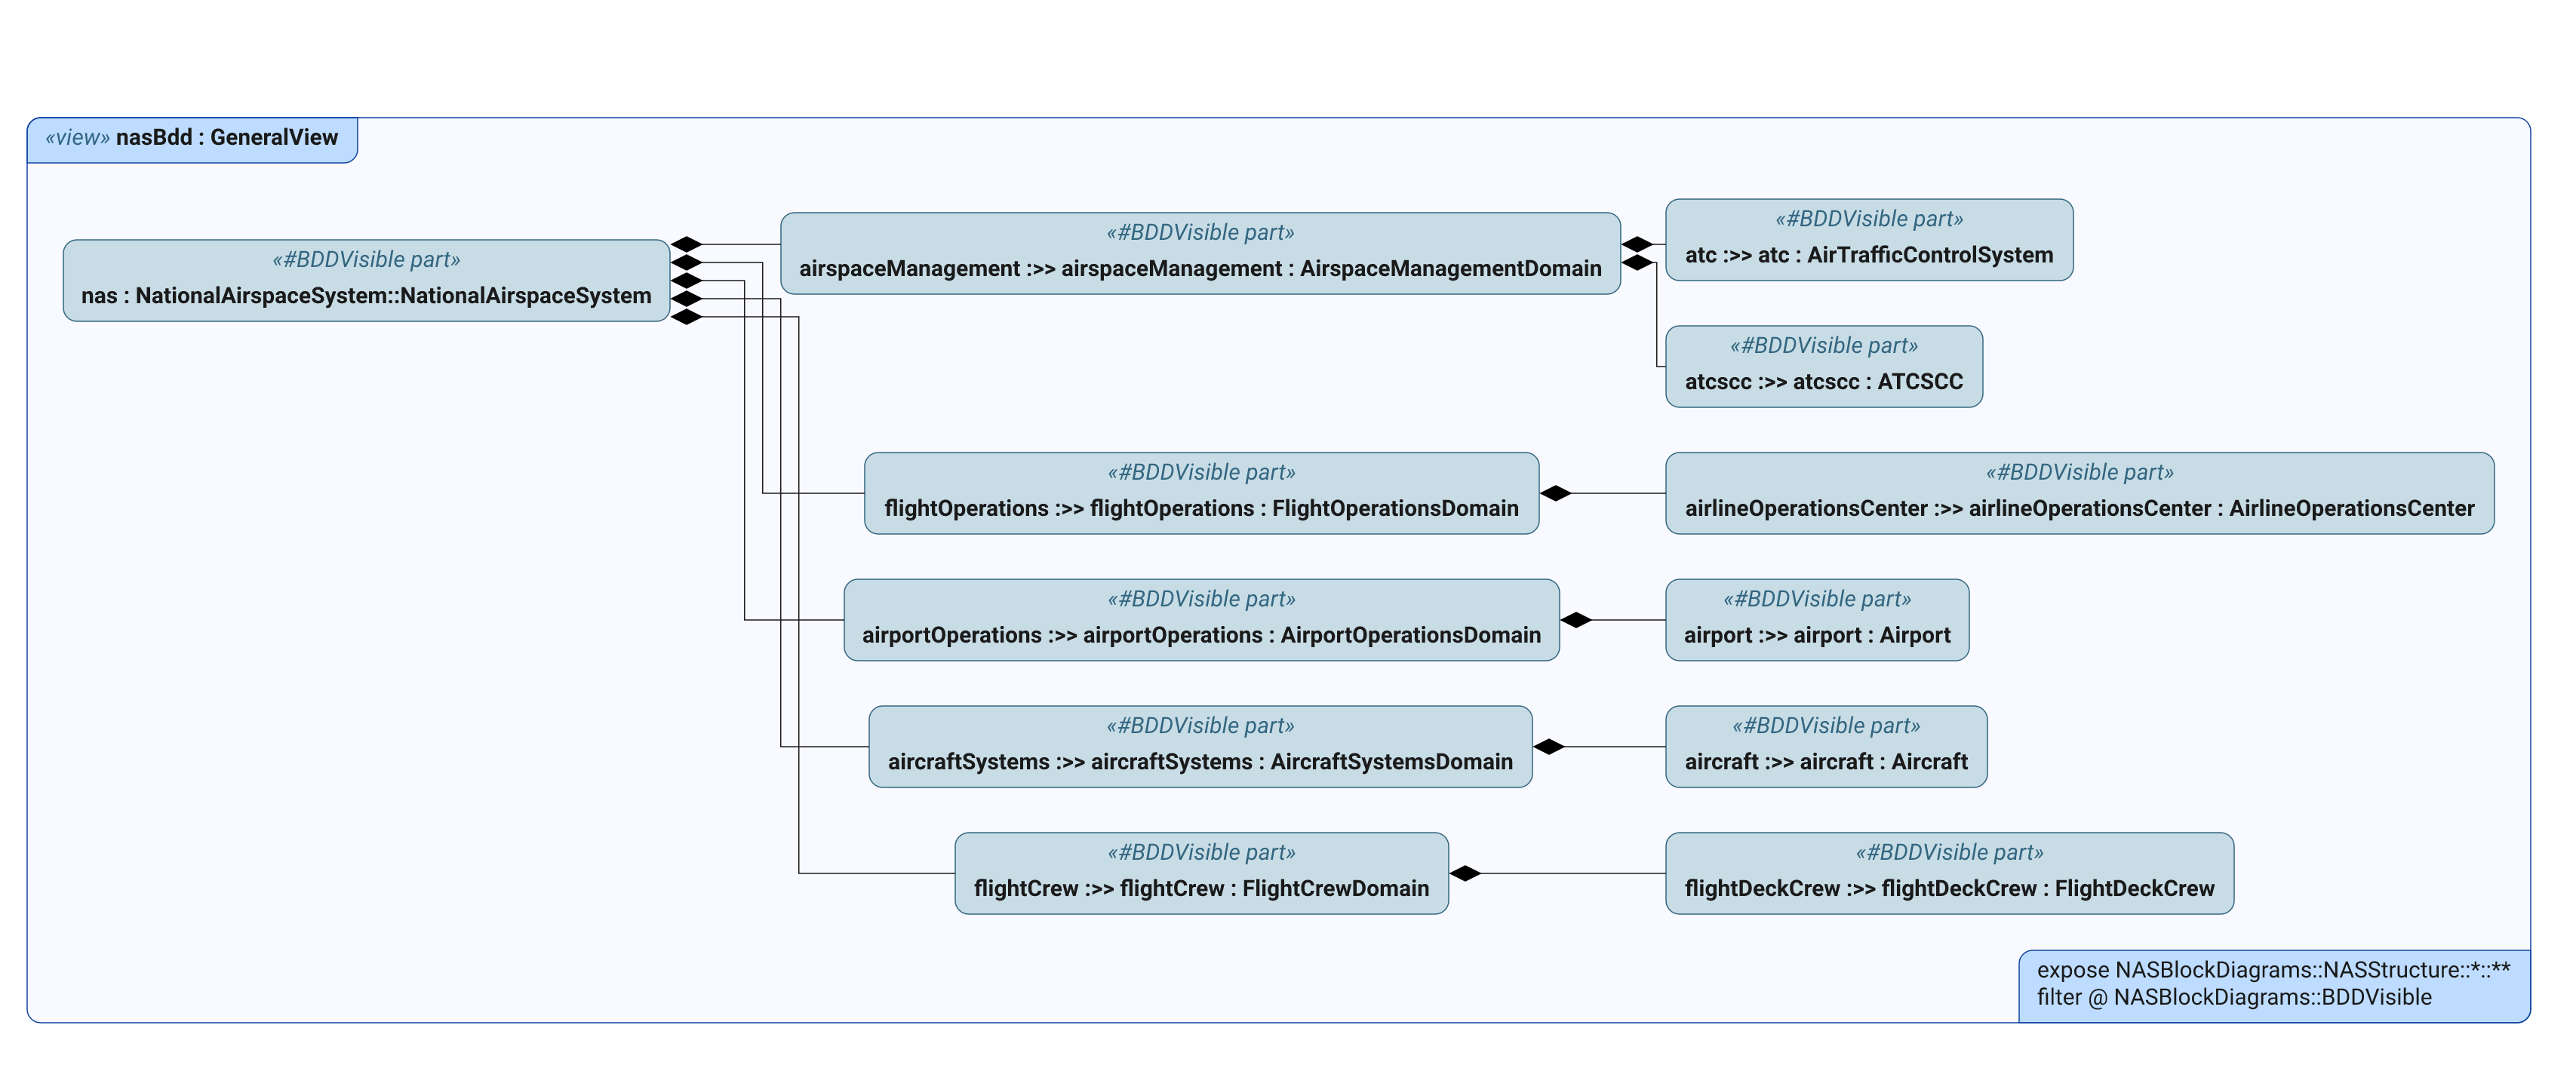
\includegraphics[width=\linewidth,height=0.8\textheight,keepaspectratio]{sysml/diagram-nasBdd}
\caption{NAS block definition diagram: the modeled domains and the context-diagram systems, composition only. View \texttt{nasBdd}; source \texttt{nas\_block\_diagrams.sysml}; rendered 2026-10-19.}
\label{fig:sysml-nasBdd}
\end{figure}
\end{landscape}

\begin{landscape}
\begin{figure}[!htbp]
\centering
\pdfimageresolution=300
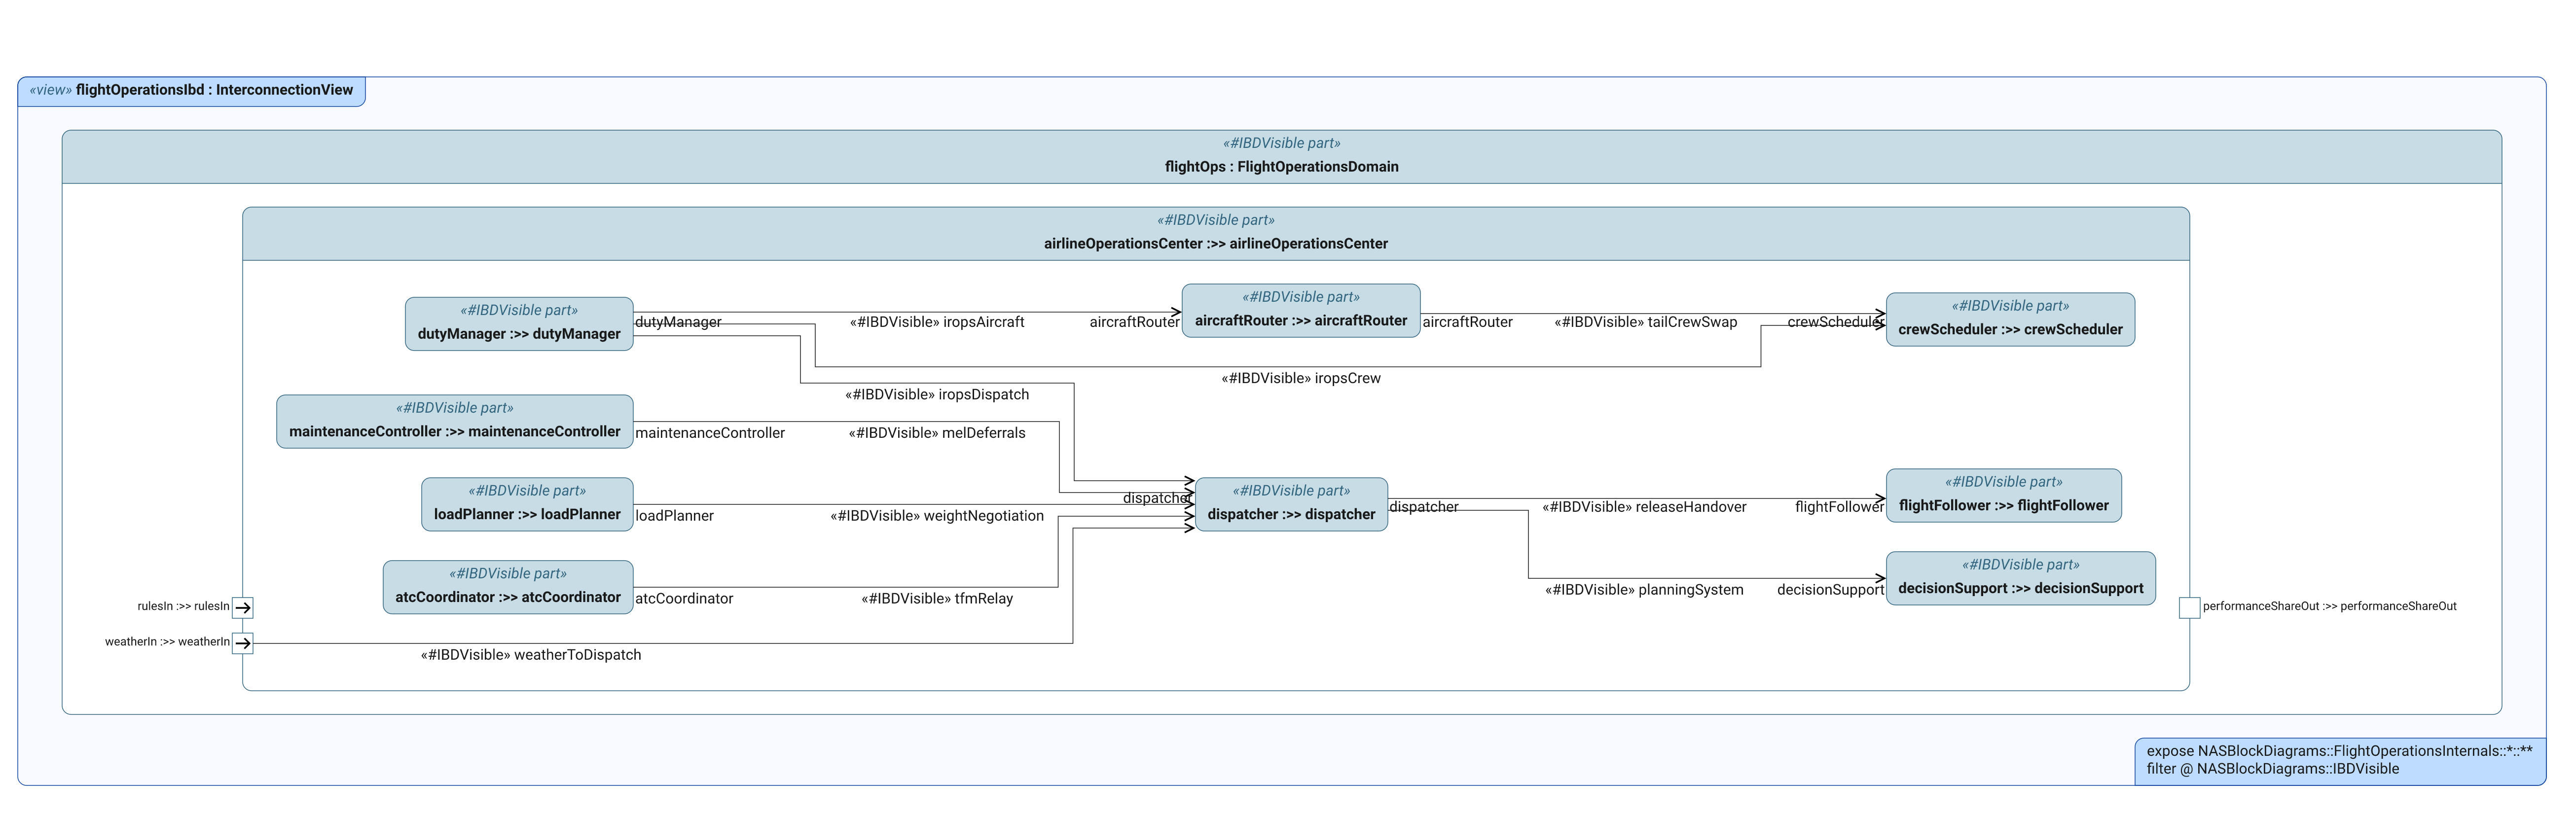
\includegraphics[width=\linewidth,height=0.8\textheight,keepaspectratio]{sysml/diagram-flightOperationsIbd}
\caption{Flight operations internal block diagram: the airline operations center's roles. View \texttt{flightOperationsIbd}; source \texttt{nas\_block\_diagrams.sysml}; rendered 2026-10-19.}
\label{fig:sysml-flightOperationsIbd}
\end{figure}
\end{landscape}

\begin{landscape}
\begin{figure}[!htbp]
\centering
\pdfimageresolution=300
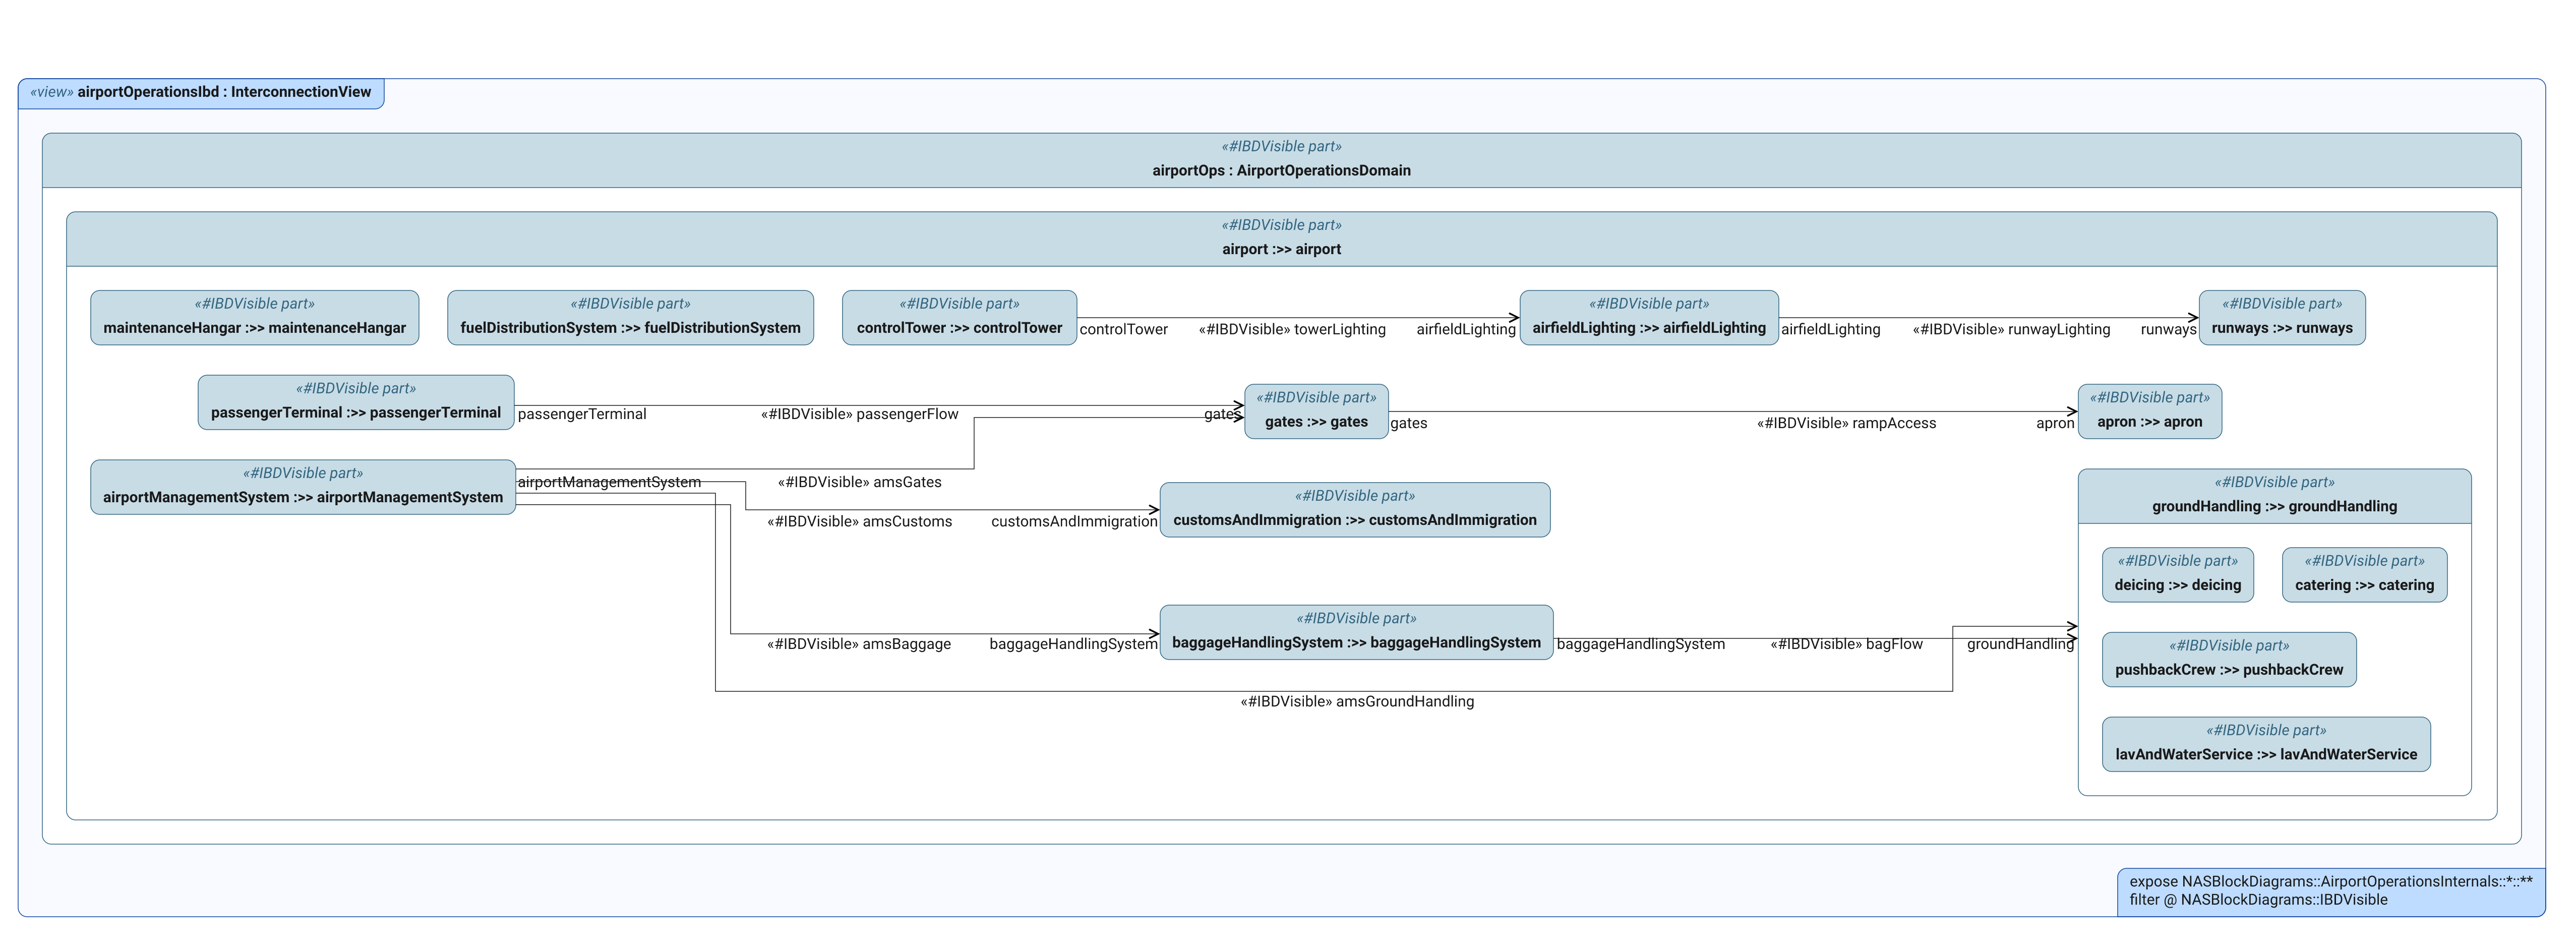
\includegraphics[width=\linewidth,height=0.8\textheight,keepaspectratio]{sysml/diagram-airportOperationsIbd}
\caption{Airport operations internal block diagram. View \texttt{airportOperationsIbd}; source \texttt{nas\_block\_diagrams.sysml}; rendered 2026-10-19.}
\label{fig:sysml-airportOperationsIbd}
\end{figure}
\end{landscape}

\begin{landscape}
\begin{figure}[!htbp]
\centering
\pdfimageresolution=300
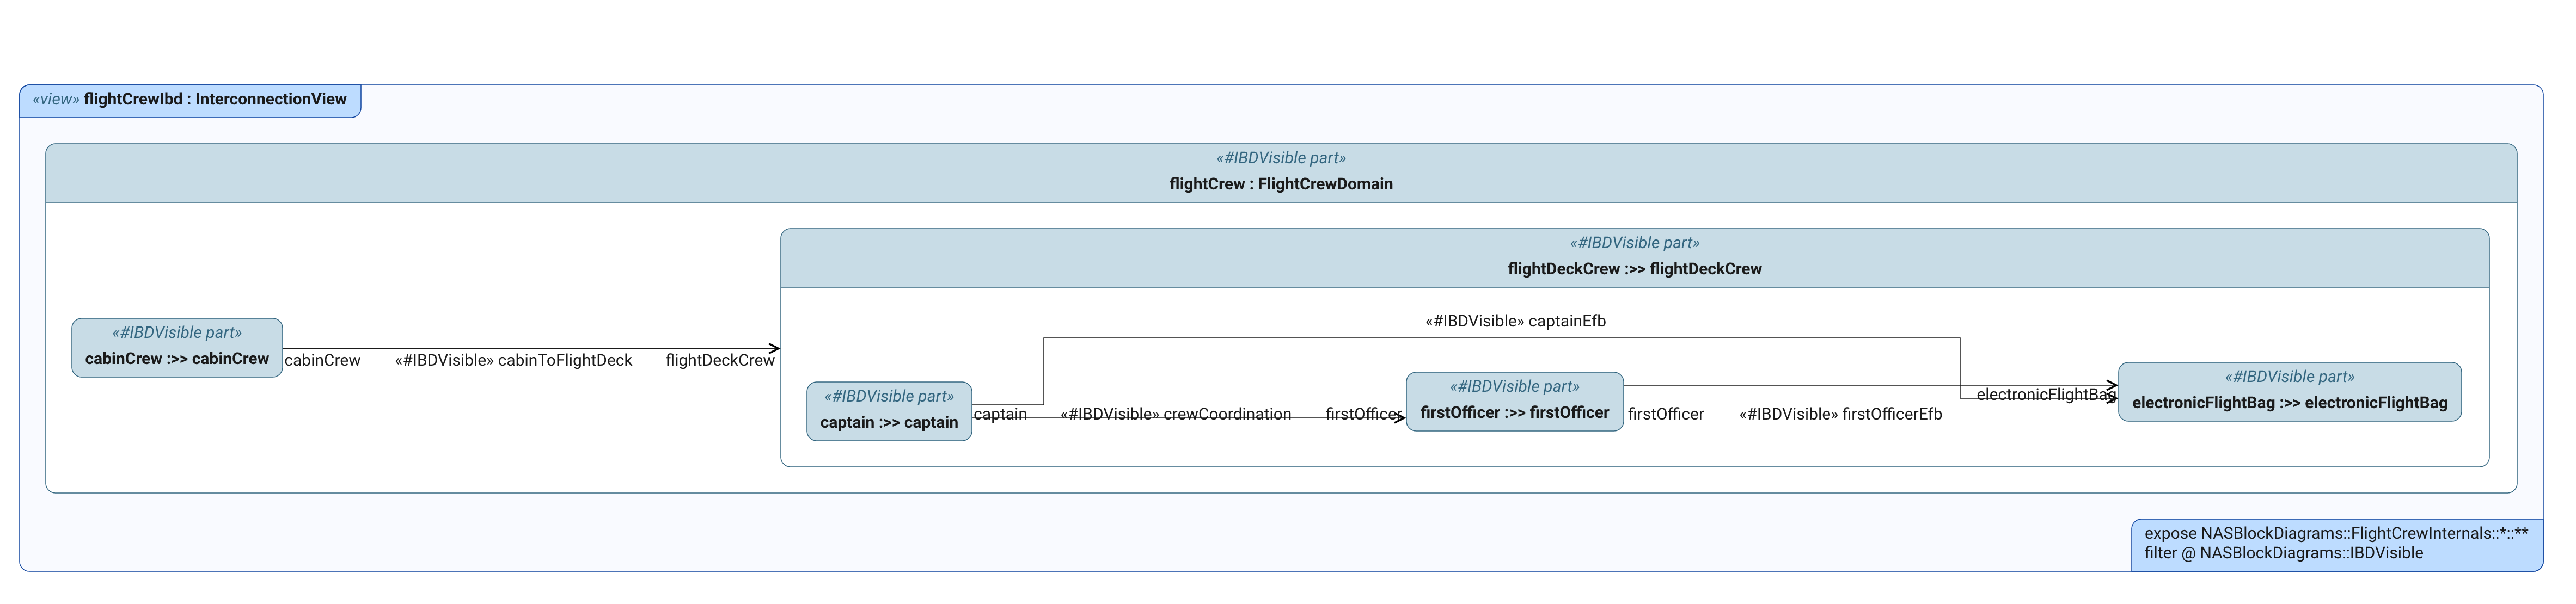
\includegraphics[width=\linewidth,height=0.8\textheight,keepaspectratio]{sysml/diagram-flightCrewIbd}
\caption{Flight crew internal block diagram. View \texttt{flightCrewIbd}; source \texttt{nas\_block\_diagrams.sysml}; rendered 2026-10-19.}
\label{fig:sysml-flightCrewIbd}
\end{figure}
\end{landscape}

\begin{landscape}
\begin{figure}[!htbp]
\centering
\pdfimageresolution=300
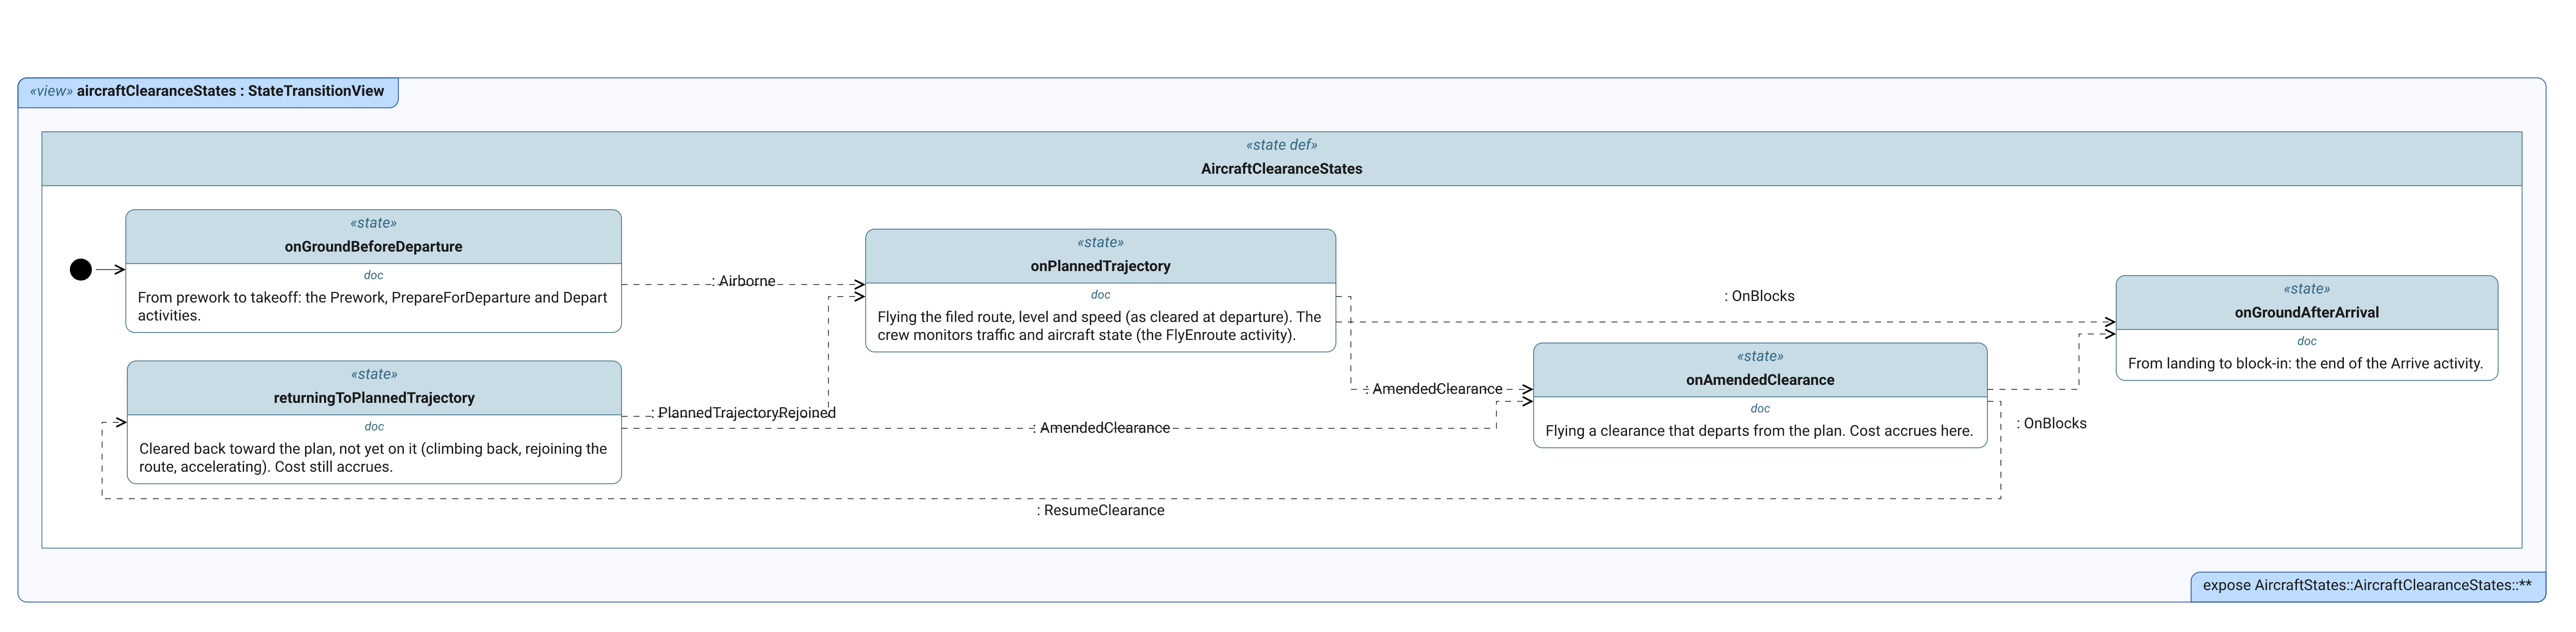
\includegraphics[width=\linewidth,height=0.8\textheight,keepaspectratio]{sysml/diagram-aircraftClearanceStates}
\caption{Aircraft state machine: the clearance the aircraft is flying, from the ground before departure to the ground after arrival. View \texttt{aircraftClearanceStates}; source \texttt{nas\_state\_aircraft.sysml}; rendered 2026-10-28.}
\label{fig:sysml-aircraftClearanceStates}
\end{figure}
\end{landscape}

\begin{landscape}
\begin{figure}[!htbp]
\centering
\pdfimageresolution=300
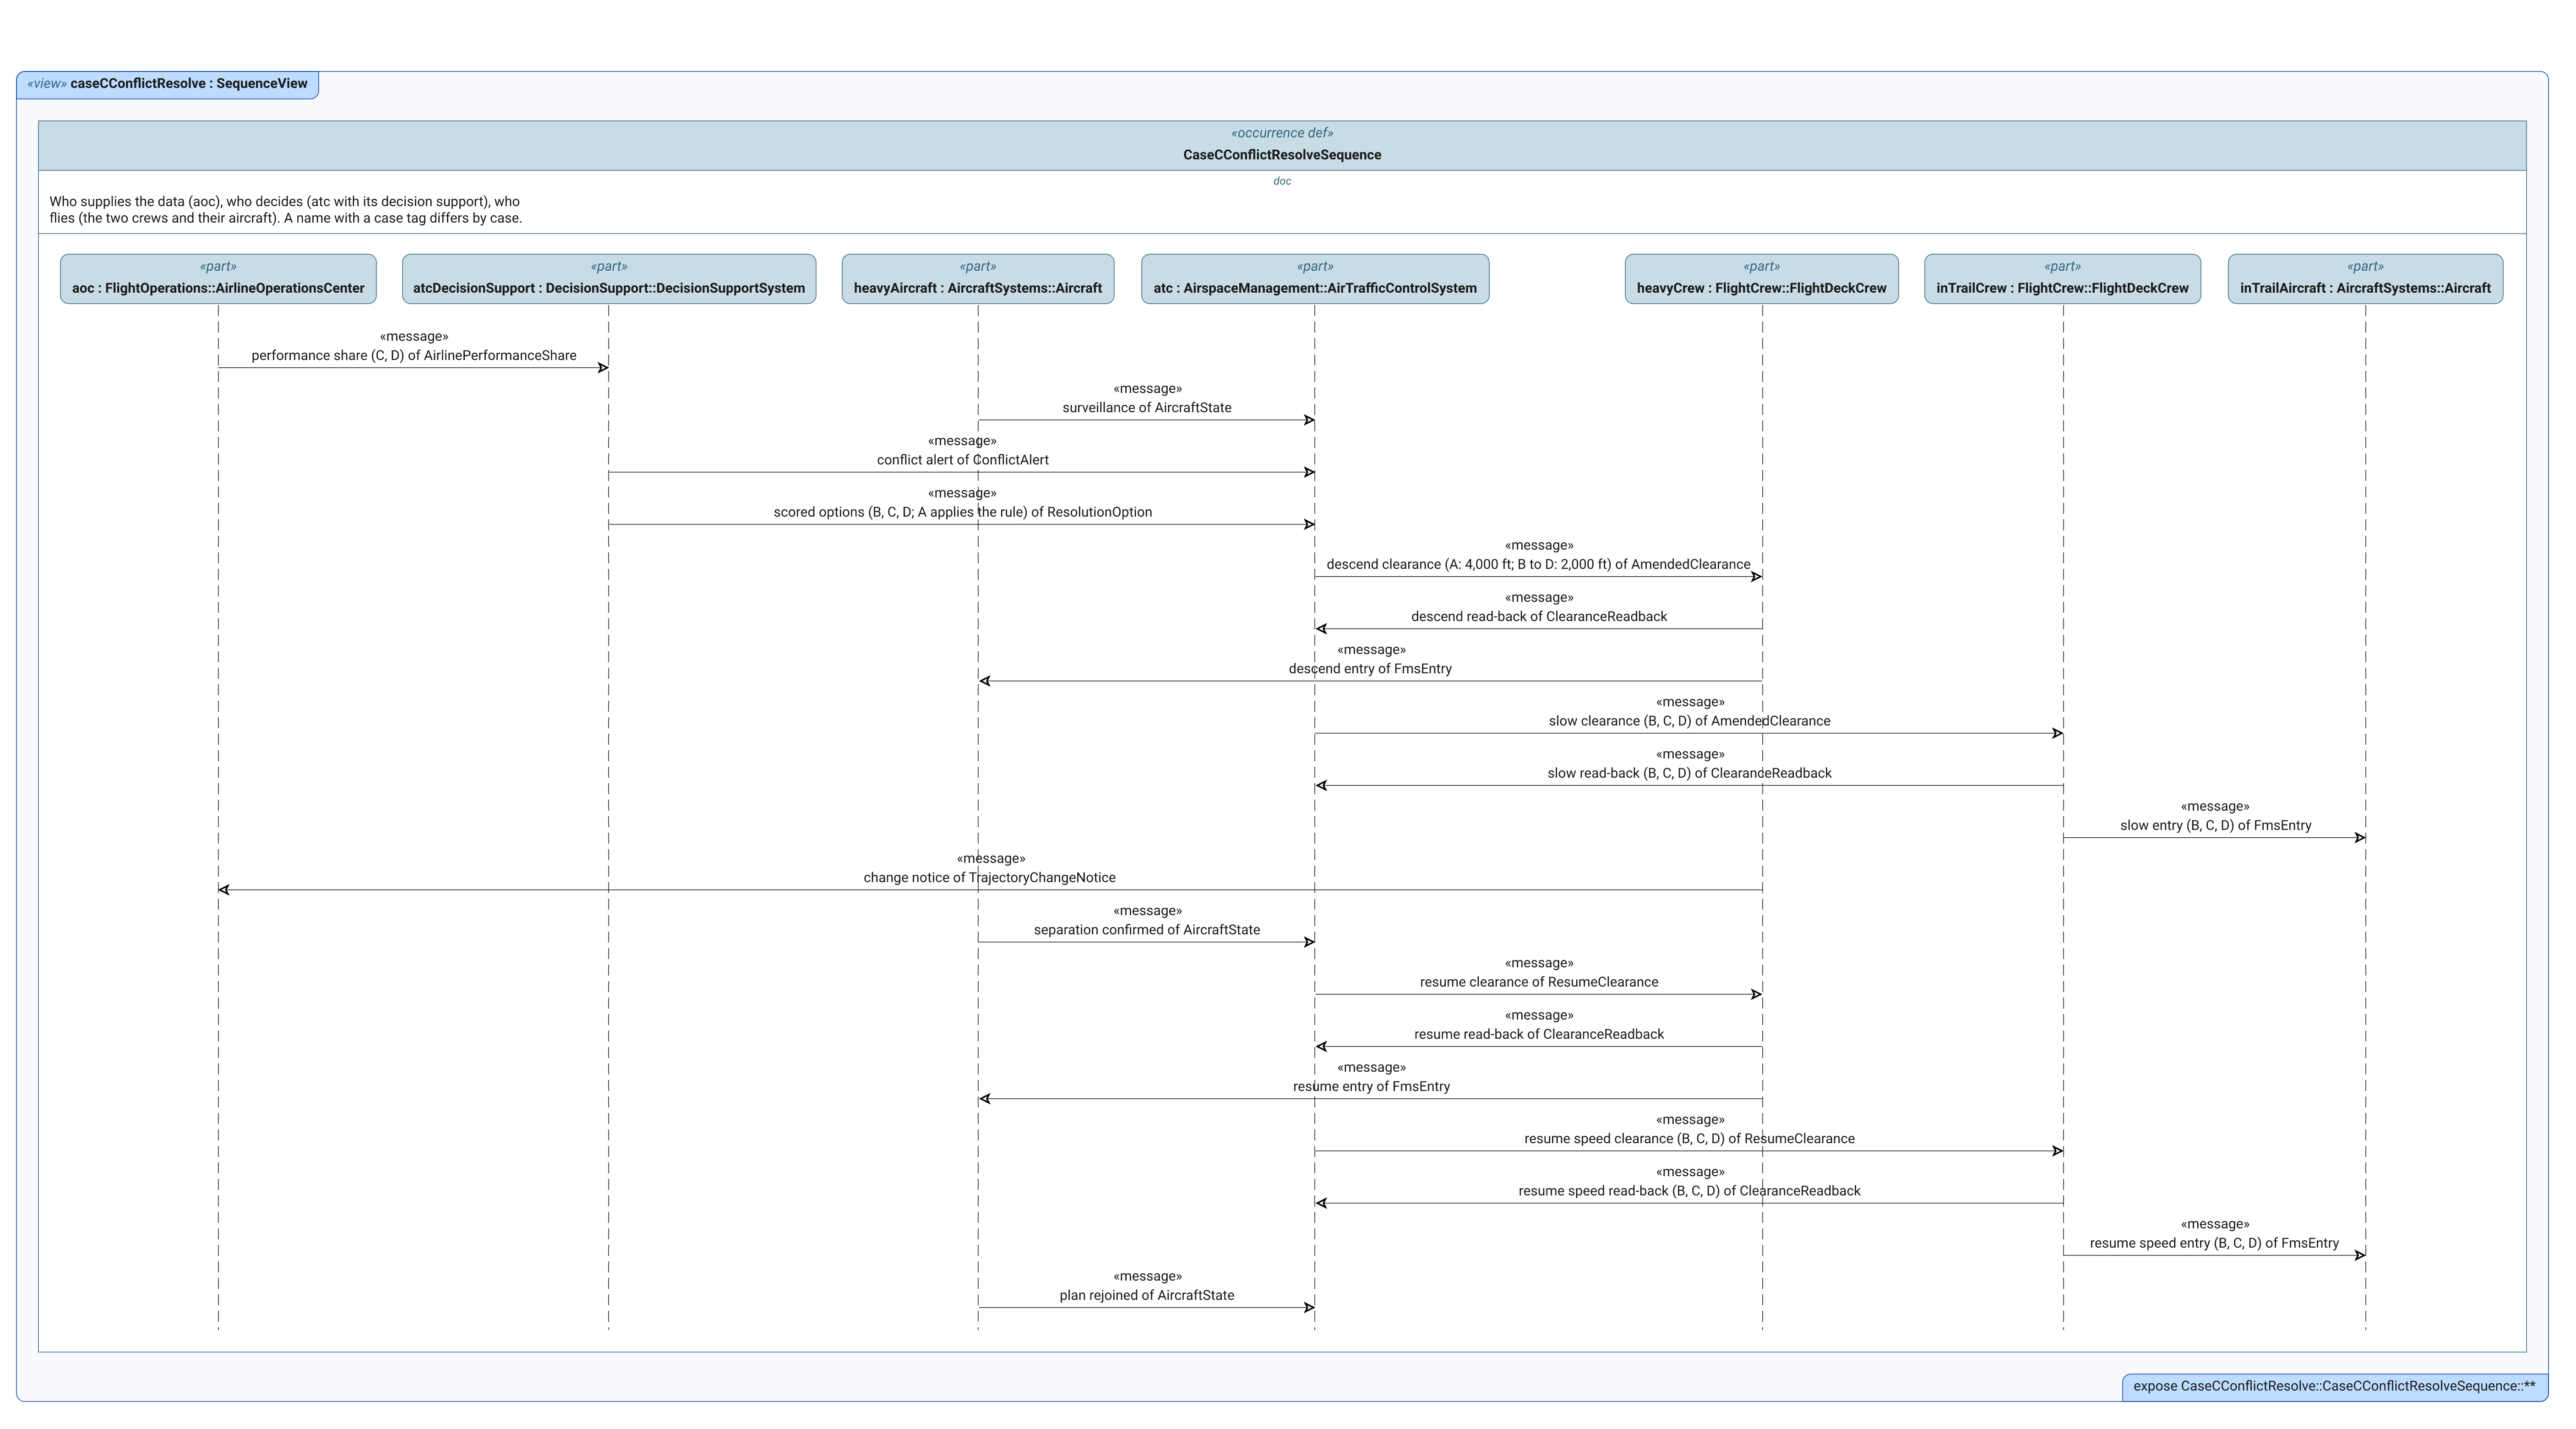
\includegraphics[width=\linewidth,height=0.8\textheight,keepaspectratio]{sysml/diagram-caseCConflictResolve}
\caption{Case C Conflict Resolve: the exchanges when ATC decision support scores the options with the airline's shared data. View \texttt{caseCConflictResolve}; source \texttt{nas\_sequence\_case\_c.sysml}; rendered 2026-10-28.}
\label{fig:sysml-caseCConflictResolve}
\end{figure}
\end{landscape}

\begin{landscape}
\begin{figure}[!htbp]
\centering
\pdfimageresolution=300
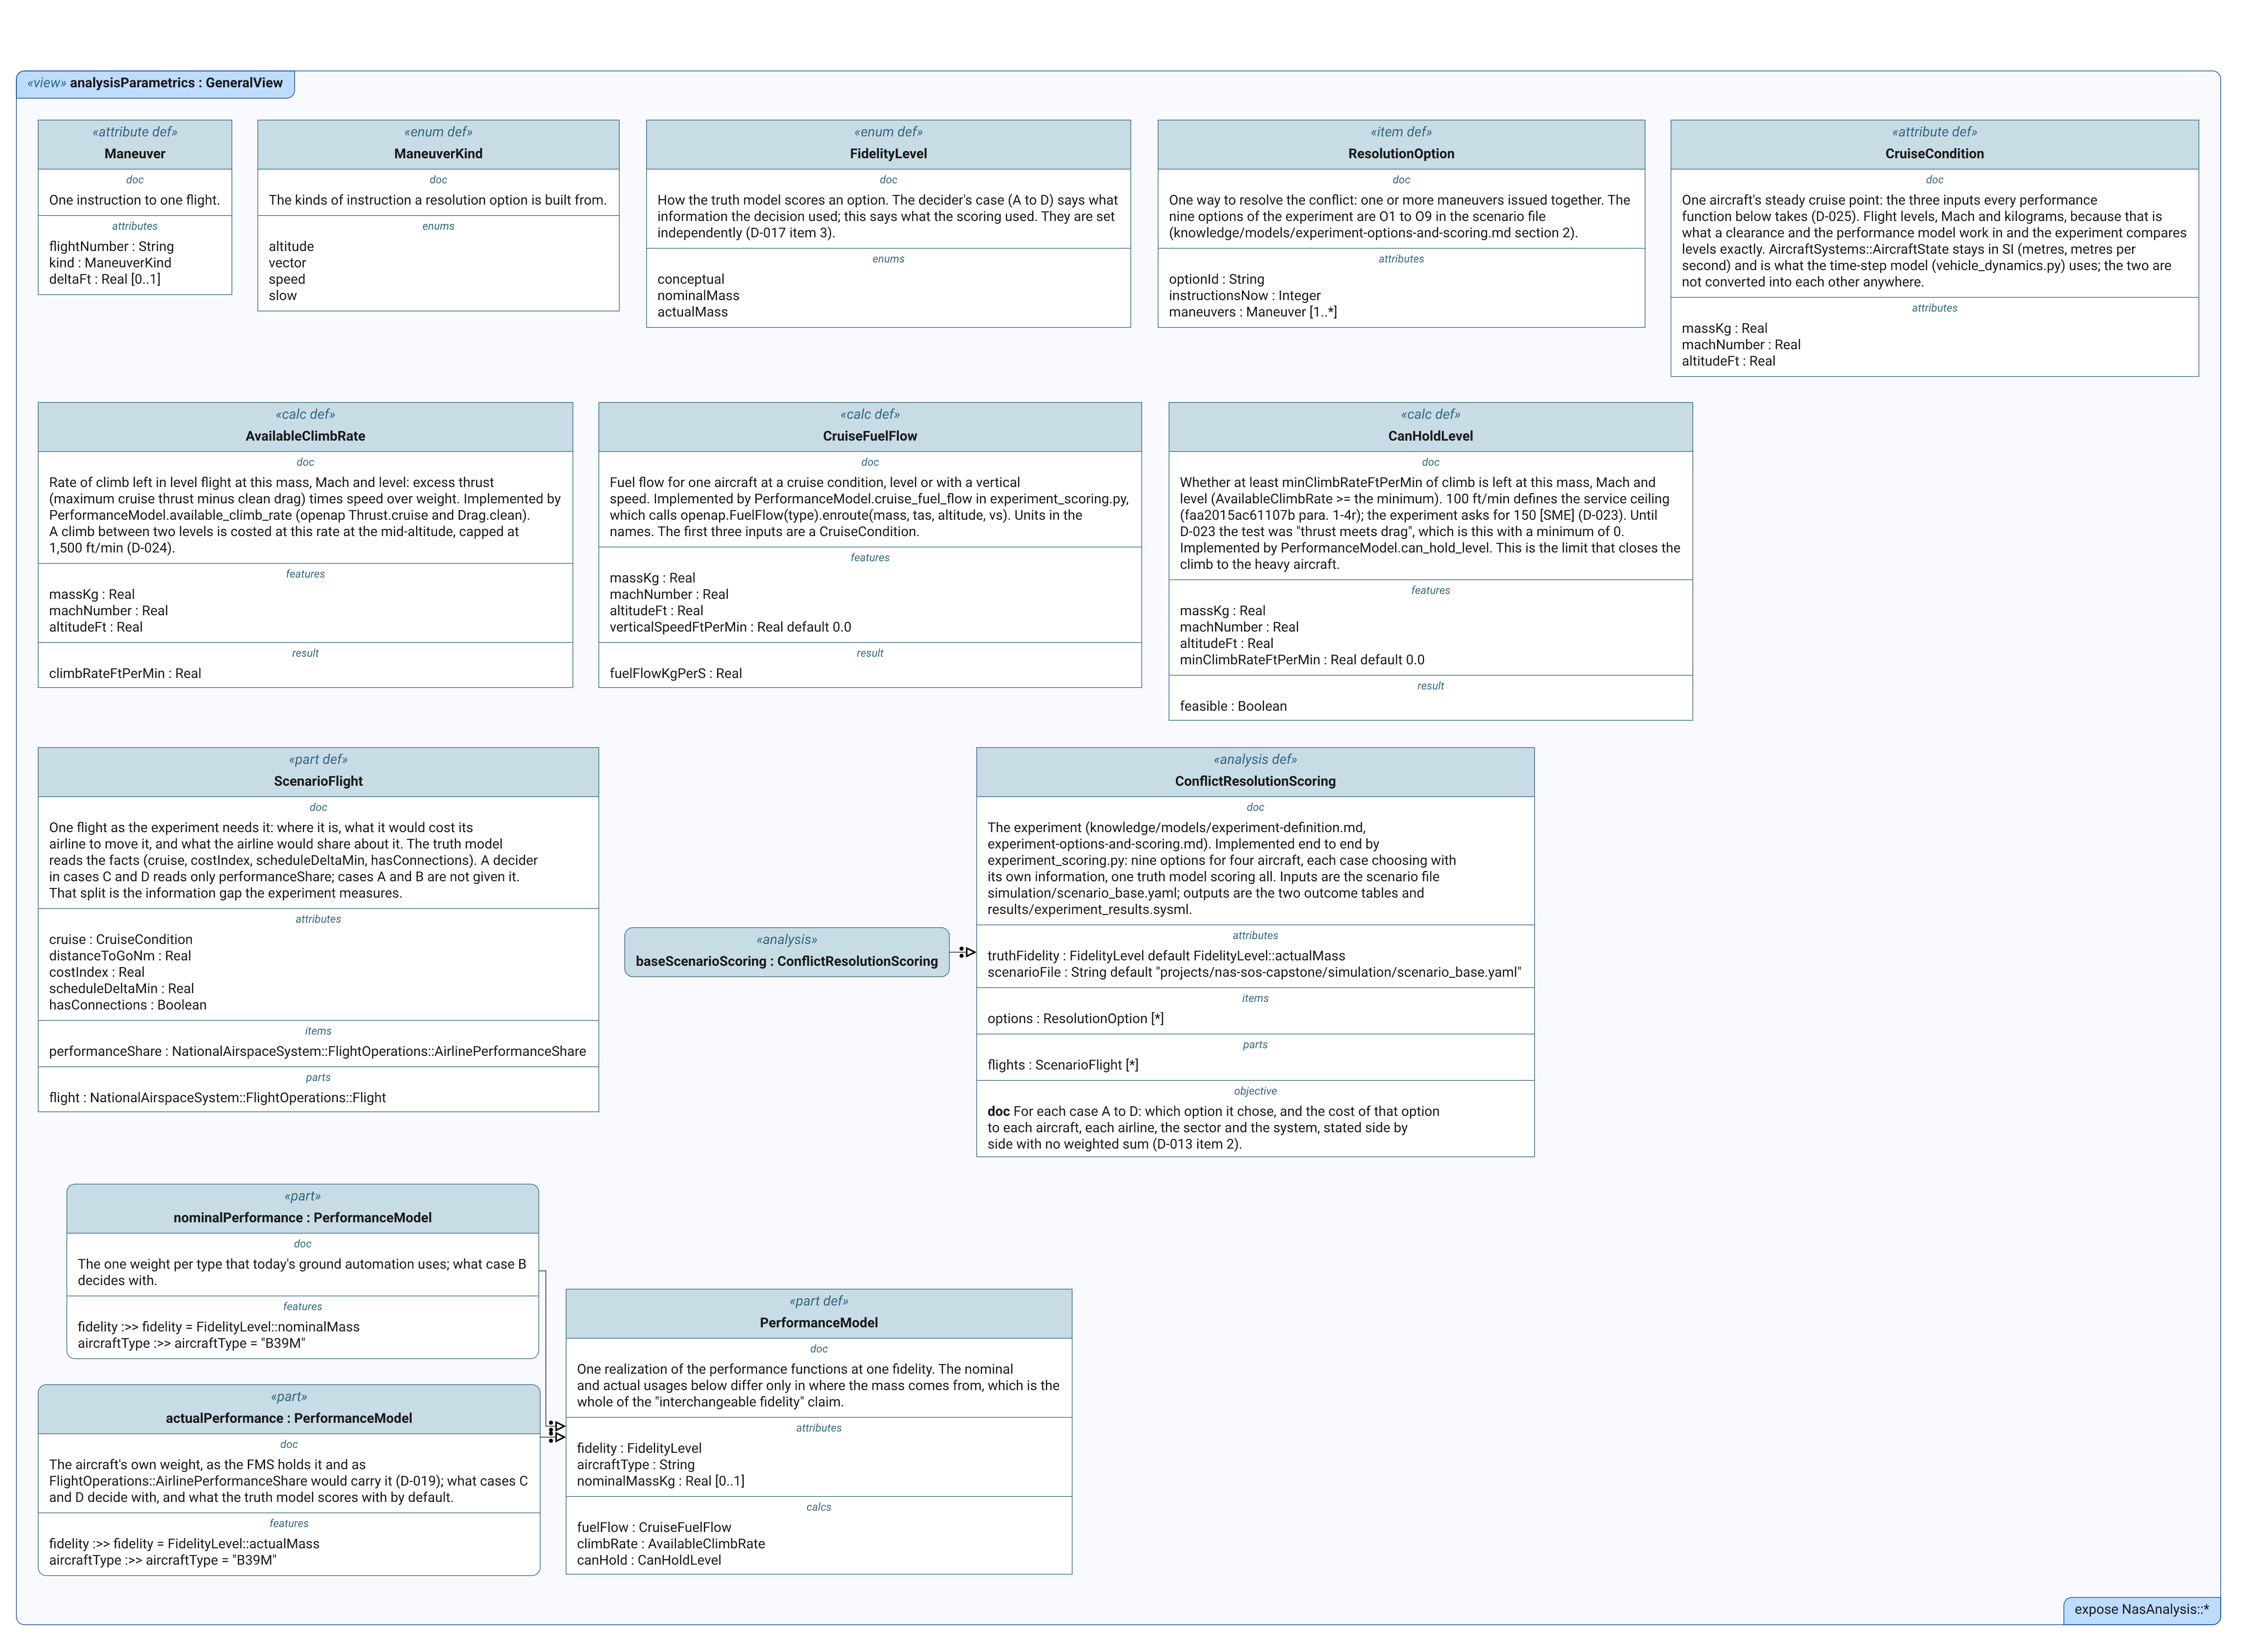
\includegraphics[width=\linewidth,height=0.8\textheight,keepaspectratio]{sysml/diagram-analysisParametrics}
\caption{Analysis definitions: the performance calculations, the two fidelity usages and the conflict-resolution scoring analysis. View \texttt{analysisParametrics}; source \texttt{nas\_analysis.sysml}; rendered 2026-10-28.}
\label{fig:sysml-analysisParametrics}
\end{figure}
\end{landscape}

% ---- end generated figures

\subsection{Full Myopic-Optimization Conflict Catalog}
\label{app:myopic}
\plantodo{S9}{All candidate conflicts not carried into the main-body
discussion or the S11--S14 demonstration scenario, each with: decision
maker, decision variable, local objective/constraints, affected
stakeholders, externalized costs, SoS consequence, and information needed
to recognize the consequence.}

\subsection{Optimization Experiment Detail}
\label{app:optimization}
\plantodo{S11, S12}{Full experiment matrix, constituent-model validation
notes, and any sensitivity-analysis detail not included in
Section~\ref{sec:results}.}

% ---- Placeholders added 2026-10-09 (AI-drafted scaffolding, not report prose).
\plantodo{S11}{Full options table: for each of the ten options, the
maneuver per aircraft, instructions now, follow-up later, and what the
decider must know to use it. Draft in
\texttt{knowledge/models/experiment-options-and-scoring.md} \S2.}

\plantodo{S11, S12}{Every option scored at four levels (the table from which
each case picks one row), the per-viewpoint cost statements with their
symbols defined, and the table of abstractions with reason and risk.}
% ---- end placeholders 2026-10-09

\subsection{Generative AI Use Disclosure}
\label{app:genai}

Generative AI was used as an assistant throughout this project. VS Code was the primary environment in which content was created, and the Claude Code extension (Anthropic) [cite] provided guidance, feedback, and draft content within it. Before that, two ChatGPT (OpenAI) [cite] conversations helped shape the project's direction. They were part of the reasoning that moved it from a trajectory-optimization study to the NAS modeled as a system of systems, with optimization as one capability inside the architecture. All AI-drafted content was reviewed and modified as needed to reflect my own views, understanding, and work.

Beyond drafting content, AI was used as a guide in three ways. It supported schedule and progress management against the course milestones. It gave technical guidance. And it critiqued the work, sometimes in deliberately demanding reviewer roles. AI gave initial reviews of all sources I identified and downloaded, to help me prioritize my own reading. After I read and marked up a source, AI extracted my markings and folded them into a library of sources and excerpts that I drew on while writing. As I wrote report sections, I asked AI for reviews, modifications, critiques, and relevant sources and excerpts.

The project's engineering content was produced the same way: AI drafted, and I reviewed, usually by hand, on paper. AI drafted much of the SysML v2 model text and the requirements, using my own work (leveraged from prior classes and authored as part of this project) as a starting point. I printed the diagrams and requirements, marked them up by hand, and AI transcribed my markings and applied them for me to check. The requirements show the effect. AI's first draft had 27 stakeholder and 53 system requirements. Over three hand reviews I struck, reworded, or wrote requirements until the set covered only what bears on the decision studied. Links in the model carry an evidence grade, so a reader can tell a link drawn from a published source or FAA order from one drawn from my industry experience or from general knowledge.

I formulated the experiment, both conceptually and in detail. AI drafted the code that implements it, runs it, and measures its outputs. AI also wrote the supporting scripts: rendering the model's diagrams, exporting the requirements, generating this report's requirement tables, and extracting annotations from PDFs. Every scenario value used in the report was set or confirmed by me. 

This disclosure is itself an example of the process. I wrote the first version. AI checked it against the project's decision log and journals and found what it left out: the ChatGPT conversations, the extent of the model and requirements drafting, and the transcription of my hand reviews. It then drafted this revision, which I edited. As with the rest of the work, the check against the record was the useful part, and the final wording is mine.

\subsection{Source Register}
\label{app:sources}
\plantodo{S1--S4}{Reference or reproduce the evidence/source register
(\texttt{evidence/source-register.md}): source, publication type,
NAS lifecycle phase, systems/stakeholders addressed, architectural and
optimization evidence extracted, and confidence/limitations.}
